% $Id: infosys-poster-sample1.tex 7631 2011-04-13 18:58:36Z tkren $
%
% TU Wien - Faculty of Informatics - Institute of Information Systems
% poster template
%
% This template is using the beamer document class and beamerposter package, see
% <http://www.ctan.org/tex-archive/macros/latex/contrib/beamer/>
% <http://www.ctan.org/tex-archive/macros/latex/contrib/beamerposter/>
% <http://www-i6.informatik.rwth-aachen.de/~dreuw/latexbeamerposter.php>
%
% For questions and comments send an email to
% Thomas Krennwallner <tkren@kr.tuwien.ac.at>
%

\pdfminorversion=4 % adobe preflight wants PDF 1.4 documents

% now start with beamer and setup some defaults (t removes some extra
% spacing before the frame starts)
\documentclass[t,final,hyperref={pdfpagelabels=true}]{beamer}
\usepackage{multirow}
\usepackage[labelformat=empty]{caption}

%
% TUINFPST options:
%  - grid: add a grid in the background for aligning text and figures
%  - cropmarks: adds cropmarks for cutting the poster
%  - landscape: create a landscape poster
%
\usepackage[]{TUINFPST}
\newcommand{\naf}{{\it not}\,}

% just for the example here
\usepackage{lipsum}
\newcommand{\tuple}[1]{\ensuremath{\langle#1\rangle}}

\usepackage{subfig}%  For \NewDocumentCommand
\usepackage{xparse}%  For \NewDocumentCommand
\usepackage{calc}%    For the \widthof macro

 \newcommand*\circled[1]{%
      \tikz[baseline=(C.base)]\node[draw,circle,fill=red!10,inner sep=2pt](C) {#1};\!
    }
\newcommand{\hilightbl}[1]{\colorbox{darkblue!20}{#1}}
\newcommand{\hilightred}[1]{\colorbox{red!38}{#1}}
\newcommand{\hilightgray}[1]{\colorbox{gray!38}{#1}}
\newcommand{\hilightgreen}[1]{\colorbox{darkgreen!38}{#1}}
\usetikzlibrary{arrows,positioning,automata,decorations,fit,backgrounds}
\usepgflibrary{shapes.geometric} % LATEX and plain TEX and pure pgf 
\usetikzlibrary{shapes.geometric} % LATEX and plain TEX when using Tik Z 
\usepgflibrary{decorations.pathmorphing} % LATEX and plain TEX and pure pgf 
\usetikzlibrary{decorations.pathmorphing} % LATEX and plain TEX when using Tik Z 
\usepgflibrary{decorations.text} % LATEX and plain TEX and pure pgf 
\usetikzlibrary{decorations.text} % LATEX and plain TEX when using Tik Z 
\usetikzlibrary{snakes}
%\usepgflibrary{shadows} % LATEX and plain TEX and pure pgf 
\usetikzlibrary{shadows} % LATEX and plain TEX when using TikZ 
\usetikzlibrary{matrix}
\usetikzlibrary{calc}
%%%%%%%%%%%%%%%%%%%%%%%%%%%% box macros %%%%%%%%%%%%%%%%%%%%%%%%%%%%

\newcommand{\Text}{Lorem ipsum dolor sit amet, consectetur adipiscing elit. 
    Sed accumsan nulla ac ipsum elementum interdum. }

\newcommand{\tikzmark}[1]{\tikz[overlay,remember picture] \node (#1) {};}
\def\uminus{\setbox0=\hbox{$\cup$}\rlap{\hbox
    to\wd0{\hss\raise0.3ex\hbox{$\scriptscriptstyle{-}$}\hss}}\box0}
\makeatletter

\NewDocumentCommand{\DrawBox}{s O{}}{%
    \tikz[overlay,remember picture]{
    \IfBooleanTF{#1}{%
        \coordinate (RightPoint) at ($(left |- right)+(\linewidth-\labelsep-\labelwidth,0.0)$);
    }{%
        \coordinate (RightPoint) at (right.east);
    }%
    \draw[red,#2]
      ($(left)+(-2.2em,1.1em)$) rectangle
      ($(RightPoint)+(1.9em,-0.3em)$);}
}

\NewDocumentCommand{\DrawBoxWide}{s O{}}{%
    \tikz[overlay,remember picture]{
    \IfBooleanTF{#1}{%
        \coordinate (RightPoint) at ($(left |- right)+(\linewidth-\labelsep-\labelwidth,0.0)$);
    }{%
        \coordinate (RightPoint) at (right.east);
    }%
    \draw[red,#2]
      ($(left)+(-\labelwidth,0.9em)$) rectangle
      ($(RightPoint)+(0.4em,-0.3em)$);}
}
\makeatother
%%%%%%%%%%%%%%%%%%%%%%%%%%%%%%%%%%%%%%%%%%%%%%%%%%%%%%%%
\newcommand{\la}{\leftarrow}
\newcommand{\sqs}{\sqsubseteq}
\newcommand{\dlp}{KB}
\newcommand{\dnot}{not~}
\newcommand{\datalogn}{Datalog^\neg}
\newcommand{\deq}{\mathrel{\stackrel{\scriptscriptstyle\Delta}{=}}}
\usepackage{etoolbox}

\newrobustcmd*{\myfilledtriangle}[1]{\tikz{\filldraw[draw=#1,fill=#1] (0,0) --
(1.2cm,0) -- (0.6cm,1.3cm);}}

\newrobustcmd*{\mytriangle}[2]{\tikz{\filldraw[ultra thick, dotted, draw=#1,fill=#2] (0,0) --
(1.2cm,0) -- (0.6cm,1.3cm) -- (0,0);}}

% \newrobustcmd*{\mytriangle}[2]{\tikz{\filldraw[very thick, dots=6 per 1cm, style=dotted,draw=#1,fill=#2] (0,0) --
% (0.2cm,0) -- (0.1cm,0.2cm) -- (0,0);}}
\definecolor{lightblue}{HTML}{D4E1F5}
%\definecolor{darkred}{HTML}{632E2E}

\def\green{\textcolor{green}}
%\def\red{\textcolor{red}}
% load our theme for the beamer poster
\mode<presentation>{\usetheme{kbs}}
\definecolor{mycolor}{rgb}{0.122, 0.435, 0.698}% Rule colour
\makeatletter
\usepackage{tcolorbox}
\newcommand{\mybox}[1]{%
  \setbox0=\hbox{#1}%
  \setlength{\@tempdima}{\dimexpr\wd0+13pt}%
  \begin{tcolorbox}[colframe=mycolor,boxrule=0.5pt,arc=4pt,
      left=6pt,right=6pt,top=6pt,bottom=6pt,boxsep=0pt,width=\@tempdima]
    #1
  \end{tcolorbox}
}
\def\cA{\ensuremath{\mathcal{A}}}
\def\cG{\ensuremath{\mathcal{G}}}
\def\cR{\ensuremath{\mathcal{R}}}

%
% this goes into the right title
%
 %\title[% upper part
%\begin{tabular}{c}
%  23rd International Conference on Artificial Intelligence (IJCAI'2013), Beijing, China, August
 % 3-9, 2013. 
%\end{tabular}

%]%
%{
% center part
% Data Repair of Inconsistent DL-programs \\[0.2\baselineskip]
%}
%
%\author{% lower part
%Thomas Eiter and Michael Fink and Daria Stepanova \\[0.75\baselineskip]
%  \{eiter,fink,dasha\}@kr.tuwien.ac.at%
%}
%
%\institute[]{% this does not go anywhere (yet)
%  Technische Universit{\"a}t Wien\\[0.25\baselineskip]
%  Institut f{\"u}r Informationssysteme%
%}


%
% this goes into the left title
%
% \titlegraphic{% place for logos, optionally use \insertinstitute to add \institute
%   \centering
%   
\includegraphics[width=150mm]{INF_Logo_typo_grau}

%   \vspace{2cm}

%   %\insertinstitute

%   \includegraphics[height=80mm]{logo_KBS_5_CMYK}%
% }
\definecolor{gray}{rgb}{0.4,0.4,0.4}
\definecolor{darkblue}{rgb}{0.0, 0.62,0.9}
\definecolor{cyan}{rgb}{0.0,0.6,0.6}
\definecolor{darkgreen}{rgb}{0,0.46,0}
\definecolor{darkred}{rgb}{0.5,0,0}

\newcommand{\red}[1]{\textcolor{darkred}{#1}}
\newcommand{\bl}[1]{\textcolor{blue}{#1}}
\newcommand{\gr}[1]{\textcolor{darkgreen}{#1}}
\newcommand{\mi}[1]{\ensuremath{\mathit{#1}}}


% these guys are only used in the pdf metainfo
\date[\today]{\today}
\subject{International Semantic Web Conference, 2018}
\keywords{Learning Rules from Incomplete KGs using Embeddings}

%%%%%%%%%%%%%%%%%%%%%%%%%%%% INFOSYS Poster %%%%%%%%%%%%%%%%%%%%%%%%%%%%

%
% of course you can pimp your poster and add some bling bling here
%

% play with the background colors
%\setbeamercolor{background canvas}{bg=InfosysLightGrey}

% fool around with background pictures
% \usebackgroundtemplate{%
% \includegraphics[width=\paperwidth]{logo_DBAI_5_CMYK}
% } 


% feel free to mess around with linespacing
%\usepackage{setspace}
%\singlespacing
%\onehalfspacing
%\doublespacing
%\setstretch{1.1}
%\renewcommand{\baselinestretch}{1.5}

% essentially, you can redefine and override everything here, no need
% to mess up the template ;-)

%%%%%%%%%%%%%%%%%%%%%%%%%%%%%%%%%%%%%%%%%%%%%%%%%%%%%%%%%%%%%%%%%%%%%%%%




% % single poster frame
% \begin{frame}\frametitle{foobar}

%   \begin{columns}[t]
%  \begin{column}{.5\textwidth}
% \begin{block}{1. Motivation}
%    \begin{columns}[t]
%   \begin{column}{.8\textwidth}
% \small{\begin{itemize}
% \item \bl{\textbf{Knowledge Graphs}}: huge collections of triples \\encoding un(bin-)ary facts under \textbf{\bl{O}}pen \textbf{\bl{W}}orld \textbf{\bl{A}}ssumption
% \medskip

% \item[]$\gr{\mi{\underbrace{\tuple{alice\;isMarriedTo\;bob}}_{isMarriedTo(alice,bob)},\underbrace{\tuple{mat\;type\;researcher}}_{researcher(mat)}}}$\medskip

% \item Automatically constructed, thus\\
%  \textbf{\red{incomplete}} / \textbf{\red{inaccurate}}
% \medskip

% \item Horn rule mining to \textbf{\bl{complete}} / \textbf{\bl{clean}} KGs \\
% e.g., $[$Galaraga, \emph{et al.}, 2015$]$
% \medskip

% \item \textbf{\red{But}}: exceptions are not captured by \\Horn rules, thus erroneous predictions
% \end{itemize}}
% \bigskip
% \bigskip
% \bigskip
% \begin{itemize}
% \item \textbf{\bl{Aim of this work:}}  methods for \\nonmonotonic rule learning \\from KGs under OWA
% \item \textbf{\red{Challenges: }} \textbf{\bl{OWA}}, \bl{\textbf{huge size}} of KGs
% \end{itemize}
% % \begin{beamerboxesrounded}[upper=uppercolblue,lower=lowercolblue,shadow=true]{Ensure quality of exceptions by minimizing conflicts}


% %\end{beamerboxesrounded}

%  \end{column}
%  \begin{column}{.5\textwidth}
%   \begin{picture}(1.99,1.99)
%       \put(-100,-180){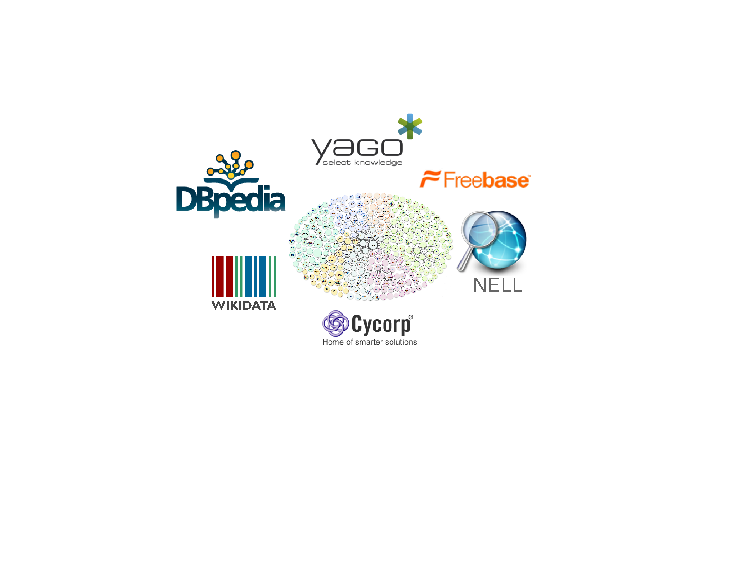
\includegraphics[width=.6\textwidth]{kb}}
%    \end{picture}
% \begin{picture}(1.99,1.99)
%       \put(-320,-630){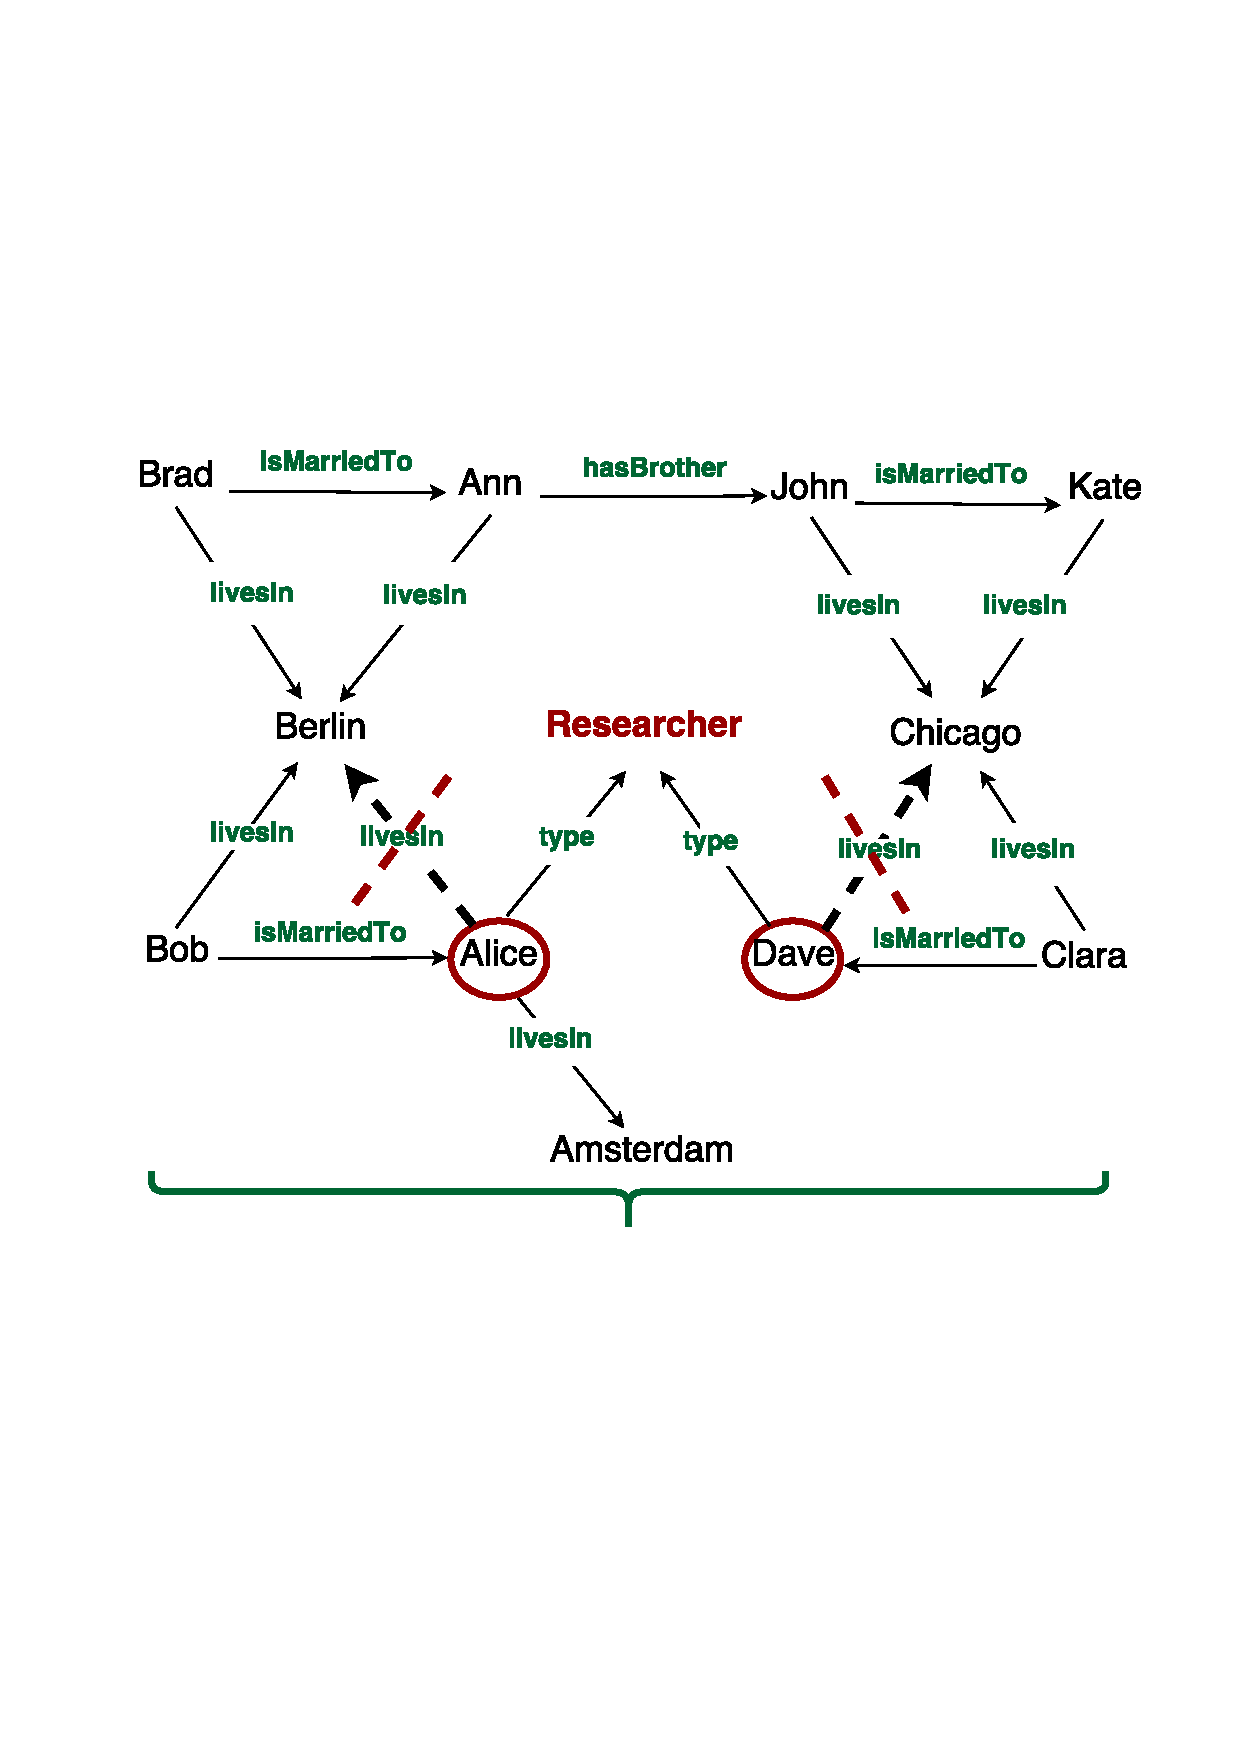
\includegraphics[width=.96\textwidth]{kg_2}}
% \end{picture}
%  \end{column}

%  \end{columns}


%  \begin{columns}[t]
%   \begin{column}{.46\textwidth}
% \bigskip
%   \end{column}
%   \begin{column}{.6\textwidth}
% \bigskip

% \scriptsize{$\mi{\gr{r:\,livesIn(X,Z)\leftarrow isMarriedTo(Y,X),livesIn(Y,Z),\,}\red{\naf\ researcher(X)}}$}
% \end{column}
%   \end{columns}

% \begin{columns}[t]
%   \begin{column}{.8\textwidth}
% \small{\begin{itemize}
% \item \textbf{\bl{Contributions: }}
% \begin{itemize}
% \item Quality-based Horn theory revision framework
% \item Exception ranking method based on cross-talk among the rules
% \item Preliminary experiments on a real-world KG
% \end{itemize}
% \end{itemize}}
% \end{column}
% \begin{column}{.5\textwidth}
% \end{column}
%   \end{columns}
% \end{block}

% \begin{block}{3. Approach Overview}
% \begin{center}
% 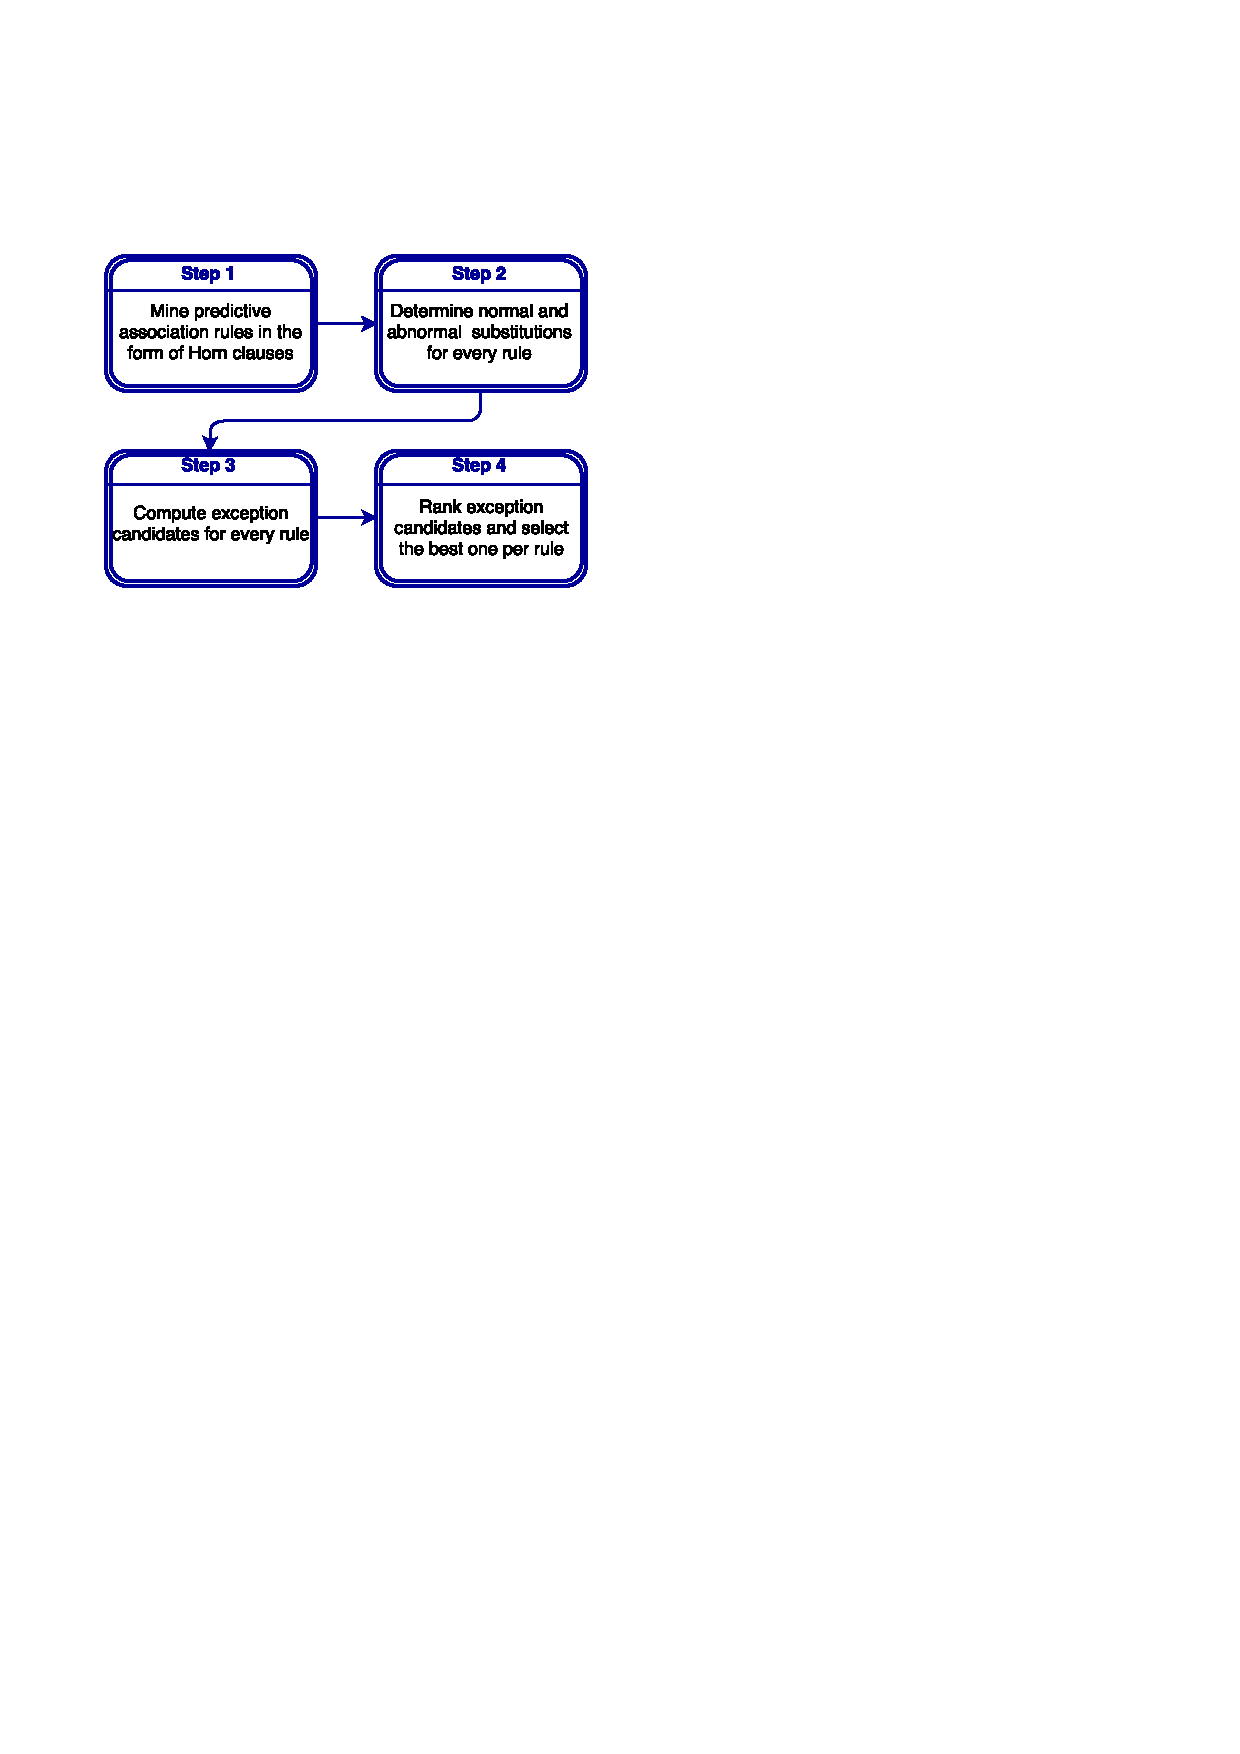
\includegraphics[width=.85\textwidth]{approach}
% \end{center}
% \end{block}
% \end{column}


% \begin{column}{.49\textwidth}
%      \begin{block}{2. Problem Statement}
% \bigskip

% \textbf{\bl{Quality-based Horn Theory Revision (QHTR)}}\bigskip

% \small{\textbf{Given:}}
% \begin{itemize}
% \item Knowledge Graph $\cG$
% \item Set of Horn rules $\gr{\cR_H}$
% \end{itemize}
% \bigskip
% \bigskip
% \bigskip

% \small{\textbf{Find:}}
%  \begin{itemize}
%  \item Nonmonotonic revision $\red{\cR_{\mi{NM}}}$, s.t.
% \medskip

%  \begin{itemize} 
%  \item{\,}\textbf{\red{conflicting predictions}} \\made by $\cR^{\mi{aux}}_{\mi{NM}}$ are minimal
% \medskip
%  \item{\,}\textbf{\red{average conviction}} is maximal\\ $conv(r,\cG) =\dfrac{1-supp(r,\cG)}{1-conf(r,\cG)}$
%  \end{itemize}
%  \end{itemize}
% \bigskip
% \bigskip
% \bigskip

% \textbf{\red{Conflicting predictions:}}

%  \small{$\cR^{\mi{aux}}_{\mi{NM}}=\left\{
% \renewcommand{\arraystretch}{1.1}\begin{array}{@{}l@{~~}l@{}}
% \mi{\gr{r_1:\,livesIn(X,Z)\leftarrow isMarriedTo(Y,X),livesIn(Y,Z),\, }\red{\naf\ res(X)}}\\
% \mi{r_1^{aux}:\,not\_livesIn(X,Z)\leftarrow isMarriedTo(Y,X),livesIn(Y,Z),res(X)}\\
% \mi{\gr{r_2:\,livesIn(X,Z)\leftarrow bornIn(X,Z)},\red{\naf\ emmigrant(X)}}\\
% \mi{r_2^{aux}:\,not\_livesIn(X,Z)\leftarrow bornIn(X,Z),emmigrant(X)}\\


% \end{array}
% \right\}
% $}
% \bigskip
% \bigskip

% $\{\gr{\mi{livesIn(c,d)},\mi{not\_livesIn(c,d)}}\}\in \cG_{\cR^{\mi{aux}}_{\mi{NM}}}$ are conflicting predictions\bigskip

% \textbf{\bl{Intuition:}} \red{researcher} might be a strong exception for \gr{$\mi{r_1}$}, but application of \gr{$\mi{r_2}$}  to \phantom{Intuition: }the KG could weaken it; less conflicts less weak exceptions



% \begin{picture}(1.99,1.99)
%       \put(520,450){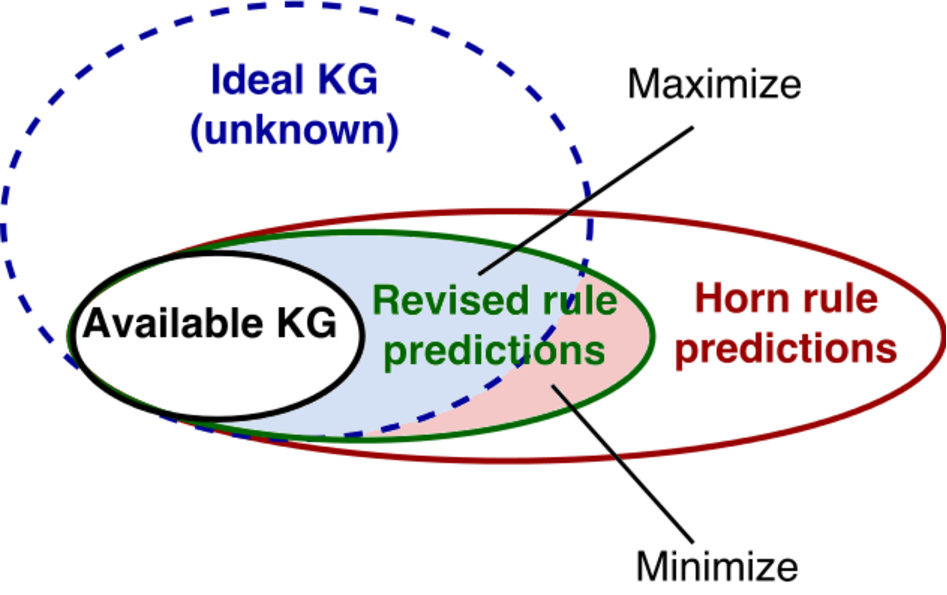
\includegraphics[width=.542\textwidth]{big_pic}}
% \end{picture}

%       \end{block}
% \vspace{-2.7cm}

%    \begin{block}{4. (Ab)normal Substitutions and Exception Candidates}
% \begin{center}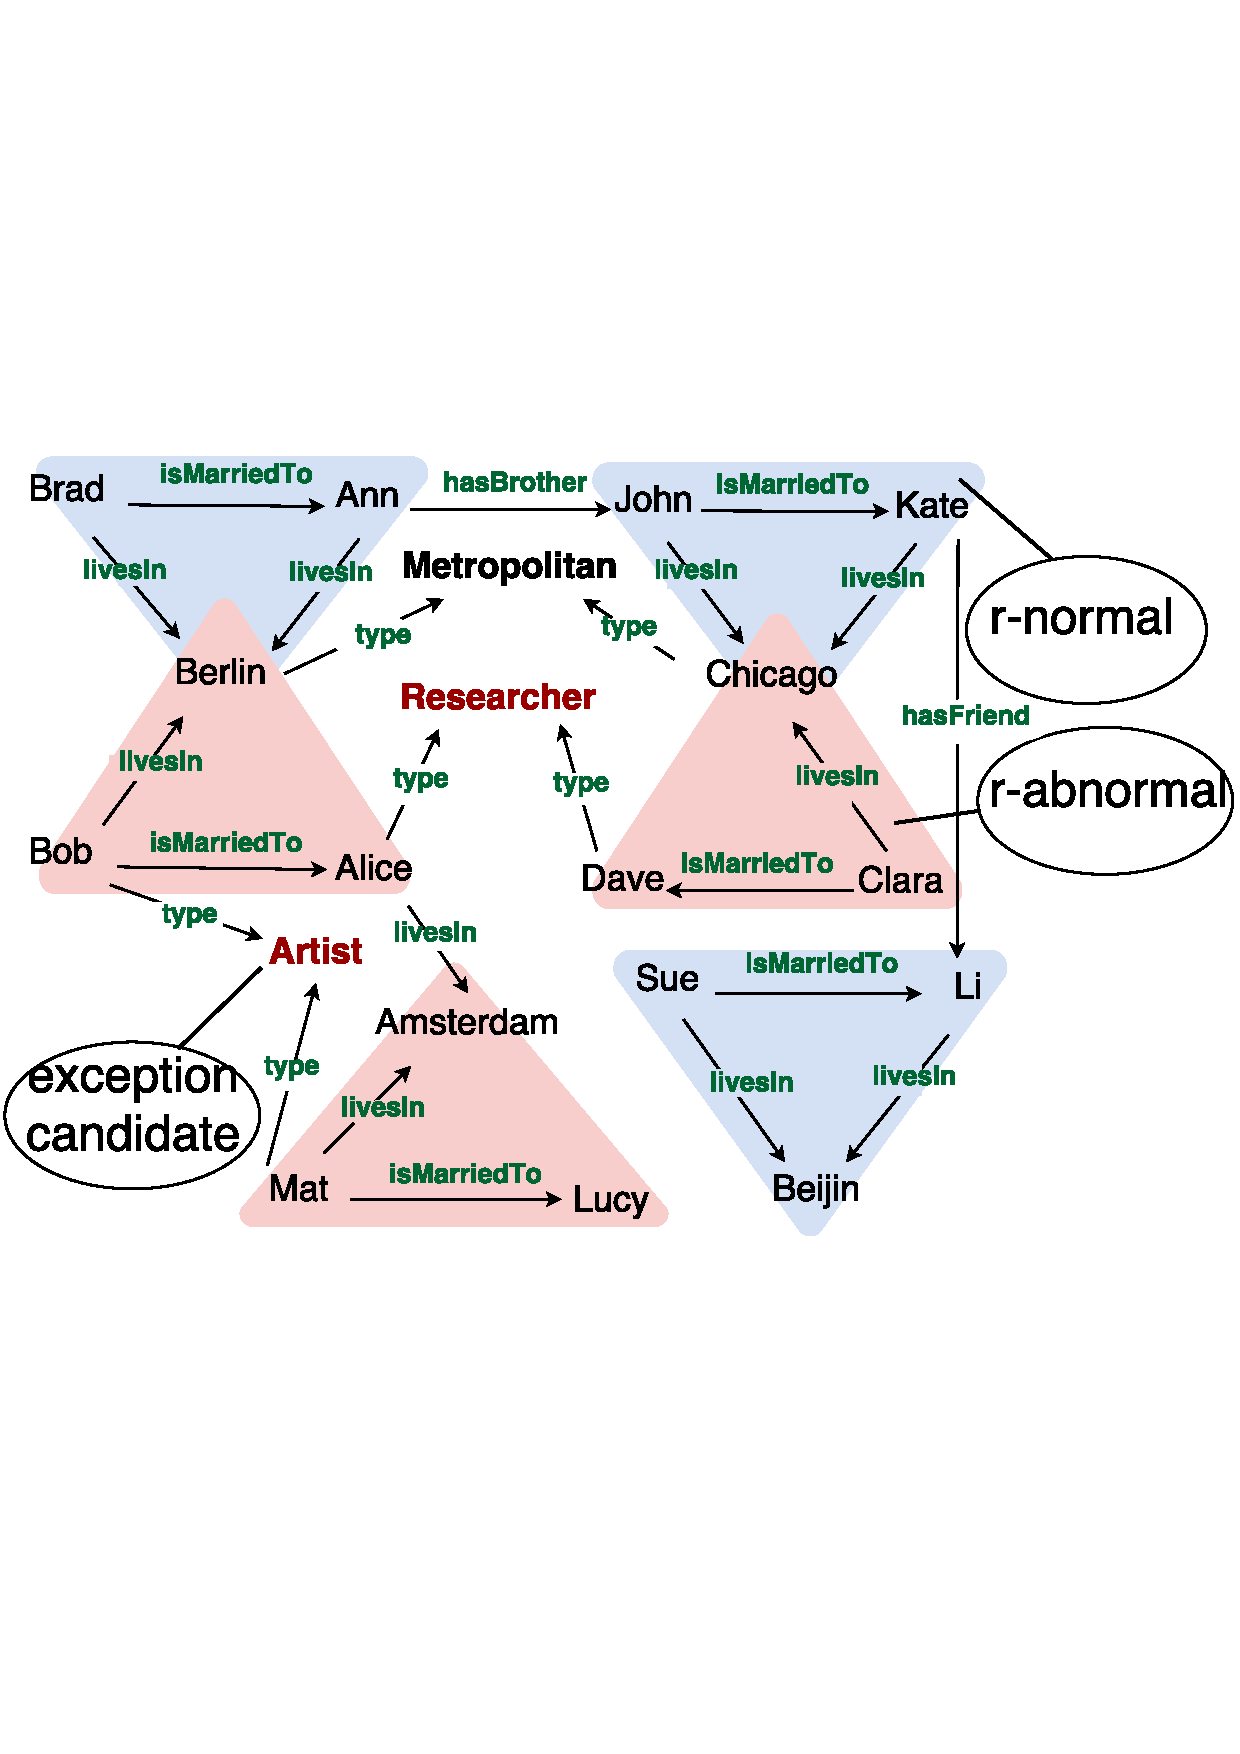
\includegraphics[width=.85\textwidth]{subs}\\
% \small{$\mi{\gr{r:\,livesIn(X,Z)\leftarrow isMarriedTo(Y,X),livesIn(Y,Z)\,}\{\underbrace{\red{\naf\,researcher(X)|\naf\,artist(Y)}\}}_{\text{\small{exception candidates}}}}$}
% \end{center}

%       \end{block}
% \end{column}
% \end{columns}
%    \vspace{-2cm}
% \begin{columns}[t]
% \begin{column}{.49\textwidth}
%      \begin{block}{5. Exception Ranking}

% \begin{center}
% $\gr{\mi{r_1} \dotsc \dotsc \dotsc} \{\red{\underline{\mathbf{e_1}}|e_2|e_3| \dotsc}\}$\\
%  $\gr{\mi{r_2} \dotsc \dotsc \dotsc} \{\red{e_1|\underline{\mathbf{e_2}}|e_3| \dotsc}\}$\\
%  $\gr{\mi{r_3} \dotsc \dotsc \dotsc} \{\red{\underline{\mathbf{e_1}}|e_2|e_3| \dotsc}\}$\\
% \end{center}
% \bigskip

% \begin{itemize}
% \item \textbf{\bl{Naive:}} pick for $r\in \cR_{H}$ a revision $r'$ with the highest $\mi{conv}(r',\cG)$

% \bigskip
% \bigskip
% \bigskip

% \item \textbf{\bl{Partial materialization:}} first cautiously materialize all rules with all of their exception candidates from $\cR_{H}\backslash r$, get a KG $\cG'$, and then pick a revision $r'$ for $r$ with the highest $\dfrac{\mi{conv(r',\cG')+conv(r'^{aux},\cG')}}{2}$

% % \only<2>{
% % $\gr{r1 \dotsc \dotsc \dotsc} \{\alert{\underline{\mathbf{e_1}},e_2,e_3, \dotsc}\}$\\
% % \hilight{$\gr{r2 \dotsc \dotsc \dotsc} \{\alert{e_1,e_2,e_3, \dotsc}\}$\\
% % $\gr{r3 \dotsc \dotsc \dotsc} \{\alert{e_1,e_2,e_3, \dotsc}\}$\\}}
% \bigskip
% \bigskip
% \bigskip

% \item \textbf{\bl{Ordered partial materialization:}} same as partial materialization, but materialize only rules ordered higher than $r$ based on $\mi{conv}$
% \end{itemize}

% \end{block}

%  \end{column}

%     \begin{column}{0.49\textwidth}
            
% \begin{block}{6. Preliminary Experiments}
% \begin{columns}
% \begin{column}{.8\textwidth}
% \vspace{-.5cm}
% \small{\begin{itemize}
% \item \bl{$\cG^i_{\mi{appr}}$}: IMDB (movie) {$\approx$}600.000 facts, {$\approx$}40 relations
% \medskip

% \item \bl{$\cG$}: random. rem. 20\% from $\cG^i_{\mi{appr}}$ for every relation
% \medskip

% \item \bl{$\cR_H$}: $\mi{h(X,Y)\leftarrow p(X,Z),q(Z,Y)}$ mined from $\bl{\cG}$
% \medskip

% \item \bl{Exception types}: $\mi{e_1(X),e_2(Y),e_3(X,Y)}$
% \medskip

% \item \bl{OPM} ranker, predictions are computed by \bl{answer set solver} dlv
% %\item $\bl{\mi{rm}}$ measure: $\mi{conv(r)=\dfrac{1-supp(r)}{1-conf(r)}}$
% \bigskip
% \end{itemize}}
% \end{column}
% \begin{column}{.5\textwidth}
% \end{column}
% \end{columns}

% \begin{table}[]
% \begin{tabular}{|r|r|r|r|r|r|r|r|r|r|}
% \hline
% \multicolumn{1}{|c|}{\multirow{3}{*}{\textbf{k}}} & \multicolumn{2}{c|}{\multirow{2}{*}{\textbf{avg. conv.}}}            & \multicolumn{1}{c|}{\multirow{2}{*}{\textbf{confl.}}} & \multicolumn{6}{c|}{\textbf{number of predictions}}                                                                                                                                                                                                           \\ \cline{5-10} 
% \multicolumn{1}{|l|}{}                            & \multicolumn{2}{c|}{}                                                & \multicolumn{1}{c|}{}                                 & \multicolumn{2}{c|}{\textbf{$\cR_{\mi{H}}$}}                                           & \multicolumn{2}{c|}{\textbf{$\cR_{\mi{NM}}$}}                                          & \multicolumn{2}{c|}{\textbf{$\cR_{\mi{H}}$ not $\cR_{\mi{NM}}$}}                                                        \\ \cline{2-10} 
% \multicolumn{1}{|c|}{}                            & \multicolumn{1}{c|}{\textbf{$\cR_{\mi{H}}$}} & \multicolumn{1}{c|}{\textbf{$\cR_{\mi{NM}}$}} & \multicolumn{1}{c|}{\textbf{$\cR_{\mi{NM}}$}}                     & \multicolumn{1}{c|}{\textbf{all}} & \multicolumn{1}{c|}{\textbf{in $\cG_{\mi{appr}}^i$}} & \multicolumn{1}{c|}{\textbf{all}} & \multicolumn{1}{l|}{\textbf{in $\cG_{\mi{appr}}^i$}} & \multicolumn{1}{c|}{\textbf{false} $\checkmark$} & \multicolumn{1}{c|}{\textbf{in $\cG_{\mi{appr}}^i$}} \\ \hline
% 5                                                 & 4.08                             & 6.16                              & 0.28                                                  & 345                               & 161                                    & 331                               & \hilightbl{156}                                    & \hilightgray{0}                                                  & \hilightgreen{14}                                             \\
% 10                                                & 2.91                             & 4.21                              & 0.08                                                  & 2178                              & 456                                    & 2118                              & \hilightbl{450}                                    & \hilightgray{27}                                                 & \hilightgreen{33}                                             \\
% 15                                                & 2.5                              & 3.42                              & 0.09                                                  & 3482                              & 629                                    & 3348                              & \hilightbl{622}                                    & \hilightgray{86}                                                 & \hilightgreen{48}                                             \\
% 20                                                & 2.29                             & 3.0                               & 0.13                                                  & 5278                              & 848                                    & 5046                              & \hilightbl{835}                                    & \hilightgray{157}                                               & \hilightgreen{75}                                            
% \\ \hline
% \end{tabular}
% \smallskip

% \caption{Top $k$ rule revision results}

% \end{table}


% \begin{picture}(1.99,1.99)
%       \put(745,470){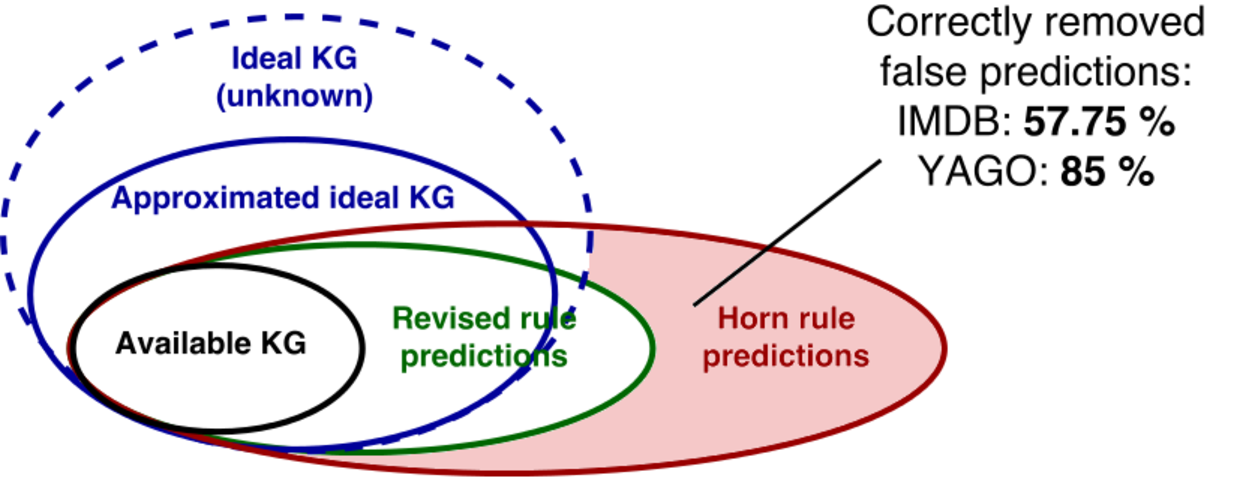
\includegraphics[width=.35\textwidth]{big_pic_exp}}
% \end{picture}
% \begin{picture}(1.99,1.99)
%       \put(895,-70){
\includegraphics[width=.15\textwidth]{imdb}}
% \end{picture}
% \bigskip
% \bigskip

% \textbf{\bl{Examples of mined rules:}}

% \bigskip

%  \begin{tabular}{l}
%  {\small
%         %\multirow{6}{*}{YAGO $\begin{cases} \\ \\ \end{cases}$}
%         $\gr{\mi{{r_1}:}\,  \mi{writtenBy(X, Z)} \,{\leftarrow}\,
%         \mi{hasPredecessor(X, Y)},\mi{writtenBy(Y, Z)},}$ \red{$ {\naf}$\,$\mi{American\_film(X)} $}}\\        
%        {\small
% $\gr{\mi{{r_2}:}\,  \mi{actedIn(X, Z)} \, {\leftarrow}\,
%         \mi{isMarriedTo(X, Y)},\mi{directed(Y, Z)},}$ \red{$ {\naf}$\,$\mi{is\_silent\_film\_actor(X)} $}} \\
    
%  \end{tabular} 
% \end{block} 

%  \end{column}
% \end{columns}
% \vspace{-10.5cm}
%  \begin{columns}[t]
% \begin{column}{.49\textwidth}
%      \begin{block}{7. References}
% \begin{thebibliography}{10}
% % \setlength{\itemsep}{0pt}
% \small{\footnotesize{
% \bibitem[\protect\citeauthoryear{Galaraga \bgroup \em et al. \egroup
%   }{2015}]{amie}
% Fast Rule Mining in Ontological Knowledge Bases with AMIE+
% {\em VLBD journal}, 2015.


%  \bibitem[\protect\citeauthoryear{Wrobel}{1996}]{theref}
%  S.~Wrobel. First Order Theory Refinement
% In proc. {\em Advances in Inductive Logic Programming}, 1996.


%   \bibitem[\protect\citeauthoryear{Gad-elrab \bgroup \em et al. \egroup}{2016}]{ours}
%   M.~Gad-elrab,D.Stepanova,J.Urbani,G.Weikum. Exception-enriched Rule Learning from Knowledge Graphs
%  In proc. {\em ISWC}, 2016.
% }}




% \end{thebibliography}

% \end{block}

%  \end{column}

%     \begin{column}{0.49\textwidth}
 
%  \end{column}
% \end{columns}

\definecolor{darkbl}{HTML}{3333B2}
\definecolor{darkgreen}{rgb}{0,0.46,0}
\definecolor{posterblue}{HTML}{DAE8FC}

\setbeamercolor{uppercolblue}{fg=black,bg=blue!10}
\setbeamercolor{lowercolblue}{fg=black,bg=blue!0}
\setbeamercolor{uppercolgreen}{fg=black,bg=green!10}
\setbeamercolor{lowercolgreen}{fg=black,bg=green!12}
\begin{document}

% single poster frame
\begin{frame}\frametitle{foobar}
\vspace{-3.8cm}

\begin{columns}
  \begin{column}{1\textwidth}
    \begin{block}{1. Motivation and Contributions}
				\begin{columns}[t]
					\begin{column}{1\textwidth}
						\vspace{-1.5em}
						\small
						\begin{center}							
						%	\item 
\bl{\textbf{Knowledge graphs}}: huge collections of positive unary and binary facts treated under \textbf{\bl{O}}pen \textbf{\bl{W}}orld \textbf{\bl{A}}ssumption (e.g. $\gr{\mi{isMarriedTo(clara,dave)},\mi{researcher(dave)}}$)
							%\item 
\bigskip

Automatically constructed, thus \textbf{\red{incomplete}}
							      $\Rightarrow$ \bl{\textbf{KG completion task}}
\bigskip
						\end{center}
					\end{column}
					\begin{column}{.5\textwidth}
					\end{column}
				\end{columns}
				\vspace{-.85cm}				
				\begin{columns}[t]					
					\begin{column}{.5\textwidth}
                                          \leftline{\;\;\;\;\;\;\;\;\;\;\;\;\;\;\;\;\;\;\;\;\bl{\textbf{Rule-based approach}}}%\end{center}
					\begin{flushleft}
\bigskip
\bigskip

\leftline{
%\begin{center}
\includegraphics[width=.7\textwidth,height=21cm]{rule_based}
\medskip
}
%\end{center}
\vspace{-1.5cm}
                                        % \begin{columns}
                                        %  \begin{column}{.47\textwidth}
					% \begin{itemize}
					% \item[\bl{+}] \bl{Interpretability, reasoning}
                                        %   \end{itemize}
                                        %   \end{column}
                                        %  \begin{column}{.47\textwidth}
                                        %   \begin{itemize}
					% \item[\red{-}] \red{Local patterns}, \red{not extendable}
					% \end{itemize}
                                        % \end{column}
                                        % \end{columns}
					\end{flushleft}
					%\end{beamerboxesrounded}
					\end{column}
					\begin{column}{.47\textwidth}
					% \begin{beamerboxesrounded}[upper=posterblue,lower=lowercolblue,shadow=true]{
\leftline{\;\;\;\;\;\;\;\;\;\;\;\;\;\;\;\;\;\;\;\;\;\;\;\;\;\;\;\;\;\;\;\;\;\;\;\;\;\;\;\;\;\;\;\;\;\;\;\bl{\textbf{Embedding-based approach}}}
%\begin{center}
\smallskip

\rightline{
\includegraphics[width=.71\textwidth, height=20cm]{embed_based}
}
%\end{center}
					\vspace{-1.5cm}
                                        % \begin{columns}
                                        %  \begin{column}{.63\textwidth}
					% \begin{itemize}
					% \item[\bl{+}] \bl{Global patterns}, \bl{extendable (e.g., text)}
                                        %   \end{itemize}
                                        %   \end{column}
                                        %   \begin{column}{.32\textwidth}
                                        %   \begin{itemize}
					% \item[\red{-}] \red{Non-interpretable}
					% \end{itemize}
                                        % \end{column}
                                        % \end{columns}
					%\end{beamerboxesrounded}
					\end{column}				

										
				\end{columns}
				\bigskip
\begin{tikzpicture}[remember picture,overlay]
		\node[] at (34,18) {%
\begin{minipage}{11cm}
				\begin{beamerboxesrounded}[upper=uppercolgr,lower=lowercolgr,shadow=true]{}
                                  \small{\textbf{\bl{+}} \bl{Interpretable}\\
					\textbf{\bl{+}} \bl{Allow for reasoning}\\
					\textbf{\alert{-}} \alert{Not extendable}\\
					\textbf{\alert{-}} \alert{Local patterns}
                                      }
									\end{beamerboxesrounded}
				\end{minipage}
					}; 
	\end{tikzpicture}

\begin{tikzpicture}[remember picture,overlay]
		\node[] at (48.5,19.5) {%
\begin{minipage}{11cm}
				\begin{beamerboxesrounded}[upper=uppercolgr,lower=lowercolgr,shadow=true]{}
                                  \small{
                                        \textbf{\alert{-}} \alert{Hard to interpret}\\
					\textbf{\alert{-}} \alert{No reasoning}\\
                                        \textbf{\bl{+}} \bl{Extendable (e.g., text)}}\\
					\textbf{\bl{+}} \bl{Global patterns}
									\end{beamerboxesrounded}
				\end{minipage}
					}; 
	\end{tikzpicture}

\begin{tikzpicture}[remember picture,overlay]
		\node[] at (41,10.7) {%
\begin{minipage}{25.6cm}
				\begin{beamerboxesrounded}[upper=uppercolbl,lower=lowercolblue,shadow=true]{\begin{center}\small{\bl{\textbf{Our approach: rule-based with embeddings support}}}\end{center}}
\bigskip

\small{
\textbf{\alert{Challenges:}}
\begin{itemize}
\item Structurally different output
\item Large embedding size
\item Large rule search space
\end{itemize}
\textbf{\bl{Contributions:}}
\begin{itemize}
\item Framework for rule learning with external sources
\item Hybrid embedding based rule  measure
\item Experiments on real world KGs
\end{itemize}
}

% \begin{columns}
% \begin{column}{.3\textwidth}
% \small{\alert{\textbf{Challenges:}}
% \begin{itemize}
% \item Difference between methods
% \item Large KG size
% \item Interaction is unclear
% \end{itemize}}
% \end{column}
% \begin{column}{.57\textwidth}
% \small{
% \textbf{Challenges:}
% \begin{itemize}
% \item Structurally difference out of methods
% \item Large embedding size
% \end{itemize}
% \textbf{\bl{Contributions:}}
% \begin{itemize}
% \item Framework for rule learning with external sources
% \item Hybrid embedding based rule  measure
% \item Experiments on real world KGs
% \end{itemize}
% }
% \end{column}
% \end{columns}

                                		\end{beamerboxesrounded}
				\end{minipage}
					}; 
	\end{tikzpicture}
	
% \put(325,-490){\bl{\textbf{Our approach:}} rule-based with embedding support
% }

		
				% \bigskip
				% \begin{columns}[t]
				% 	\begin{column}{1\textwidth}
				% 		\vspace{-3.1em}
				% 			\bigskip
				% 	\end{column}
				% 	\begin{column}{.5\textwidth}
				% 	\end{column}
				% \end{columns}

\end{block}
\end{column}
\end{columns}
\vspace{-5.5cm}

	\begin{columns}[t]
		\begin{column}{.5\textwidth}
			\begin{block}{2. Our Proposal: Rule Learning with External Sources}
\begin{itemize}
\item \textbf{Problem statement:}
\smallskip

\;\;\;\small{\textbf{Given:} $\mathcal{P}=(\cG,f)$
\begin{itemize}
\item \textbf{\bl{Knowledge graph} $\mathcal{G}$}				
\item \textbf{\bl{Probability function}} $f$: trusfulness of $\cG$'s missing facts
\end{itemize}}
\bigskip

\;\;\;\small{\textbf{Find:} Ordered set of \textbf{\bl{rules}}, which  
\begin{itemize}
\item \textbf{\bl{Describe}} $\cG$ well and \textbf{\bl{predict}} highly probable facts based on $f$
\end{itemize}}

\bigskip
\bigskip

\item \normalsize{\textbf{Our solution:}}
\bigskip

\small \bl{\textbf{Hybrid rule quality function}} to prune search space of rules $r$:   
\bl{\[\mu(r,\mathcal{P})= (1 - \lambda) \times \mu_1(r,\cG) + \lambda \times \mu_2(\cG_r,\mathcal{P})\]}
\vspace{-1cm}
						\begin{itemize}
							\item \bl{\textbf{Descriptive quality} \pmb{$\mu_1$}} of rule $r$ over $\mathcal{G}$:
							      \bl{\[\mu_1: (r,\cG) \mapsto \alpha \in  [0,1]\]}
							      $\Rightarrow$ any classical rule measure, e.g., confidence
							      \bigskip
							      \bigskip

			\item \bl{\textbf{Predictive quality} \pmb{$\mu_2$}} of $r$: trustfulness of predictions $\cG_r$ made by $r$ on $\cG$
							      \bl{\[\mu_2: (\cG_r{,}\, \mathcal{P}) \mapsto  \alpha \,{\in}\, [0,1]\]}
							      $\Rightarrow$ capture \textbf{\bl{information about missing facts}} in $\cG$ that are relevant for $r$
\bigskip

							\item \bl{\textbf{Weighting factor}} \pmb{\bl{$\lambda$}} \bl{$\in [0, 1]$} to control the distribution of $\mu_1$ and $\mu_2$
% \item \bl{\textbf{Realization of $\mu_2:$}}  

%   \bl{\[\mu(\cG_r,\mathcal{P})=\dfrac{\sum_{a\in \cG_r\backslash \cG} f(a)}{|\cG_r \backslash \cG|}\]}
						\end{itemize}	

\bigskip
\bigskip

\item \normalsize{\textbf{Realization of $f$ and $\mu_2$ relying on embeddings:}}\vspace{-.7cm}
\small{\begin{center}	\bl{\[f(fact)=0.5\times (1/subject\_rank(fact)+1/object\_rank(fact))\]}\\
\bl{$\mu_2(\cG_r,\mathcal{P}) = \dfrac{\Sigma_{fact\in \cG_r\backslash \cG}\ f(fact)}{ |\cG_r \backslash \cG|}$}
\end{center}}

%				\bigskip
%\begin{center}
%                                          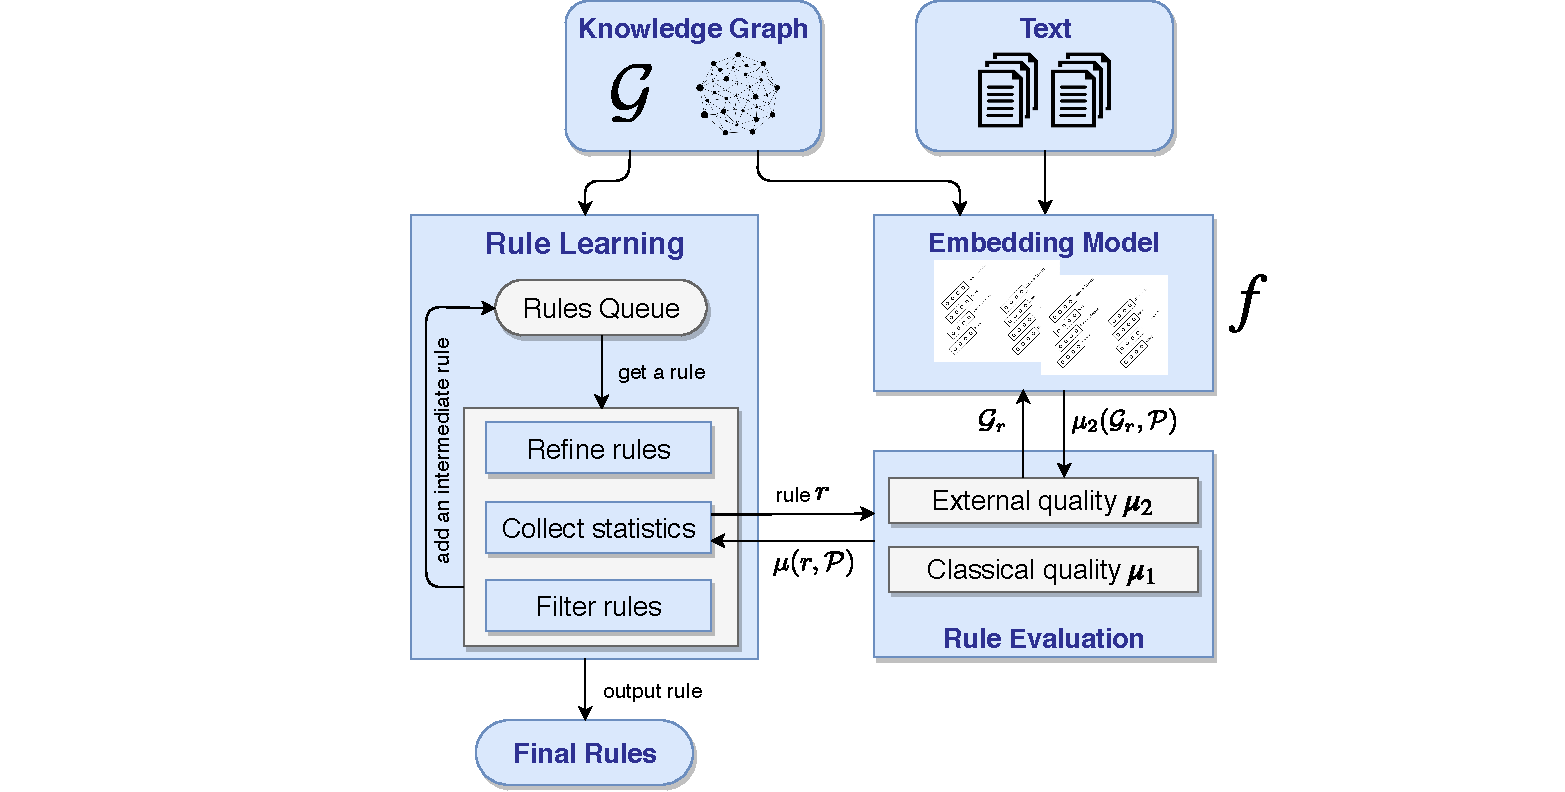
\includegraphics[width=1\textwidth]{mining}
%\end{center}
\end{itemize}
			\end{block}
			\vspace{-1.5cm}

		\end{column}
				
				
		\begin{column}{.5\textwidth}
	
			\begin{block}{3. General Architecture}
\bigskip
\bigskip

\rightline{
  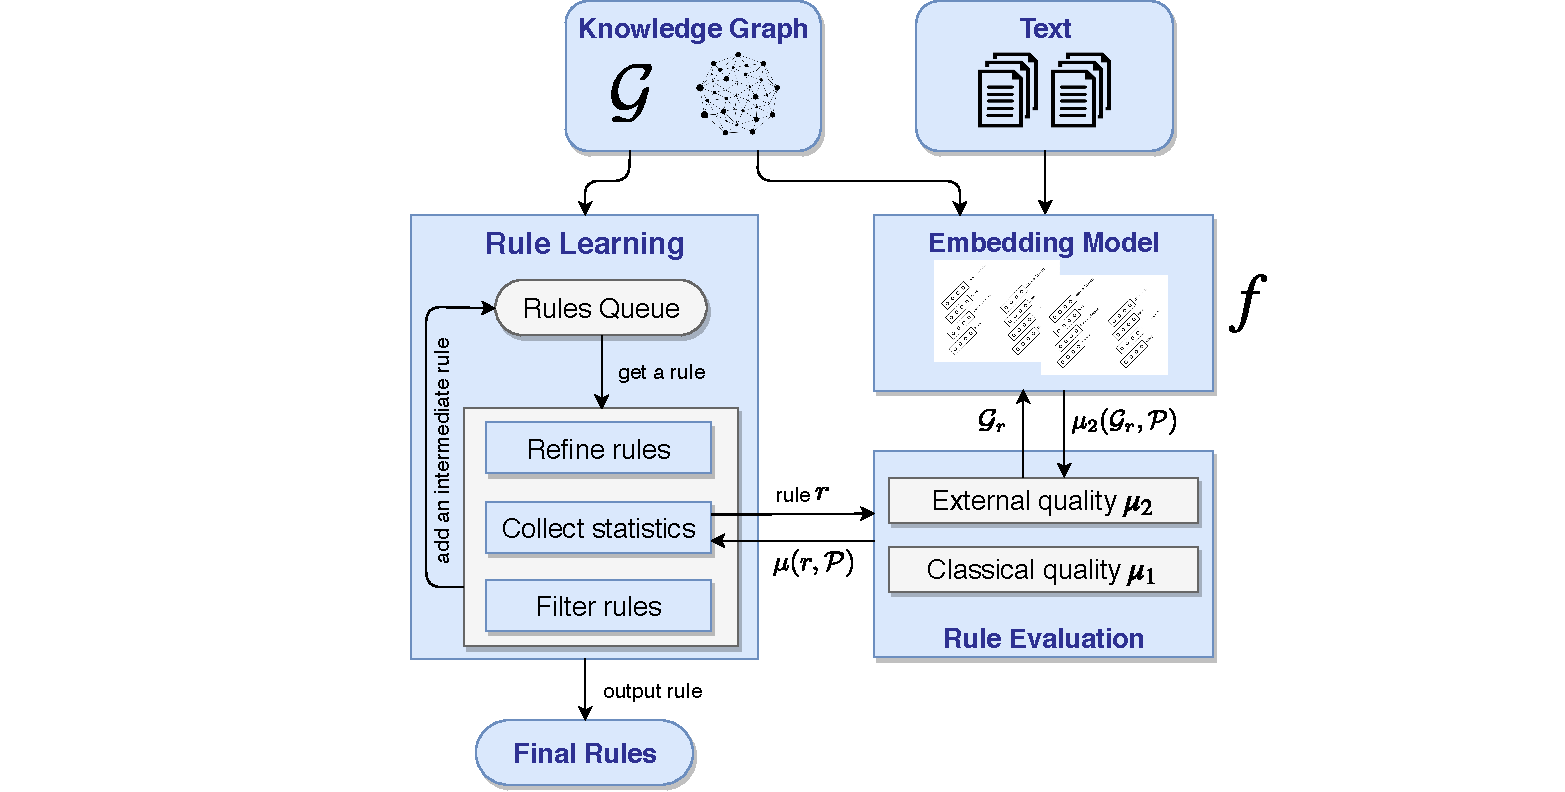
\includegraphics[width=1\textwidth]{mining}
}

			\end{block}
		\end{column}
	\end{columns}

	\begin{columns}[t]
		\begin{column}{.5\textwidth}
\vspace{-.4cm}
			\begin{block}{4. Rule Refinement}	
\bigskip

$\,\,\,$ \small{Extended AMIE [Gal{\'{a}}rraga, \emph{et al}, VLDB 2015] (additions are in blue)}:			
\bigskip
\bigskip
\bigskip
		% \begin{picture}(1.99,1.99)
% 					\put(325,-490){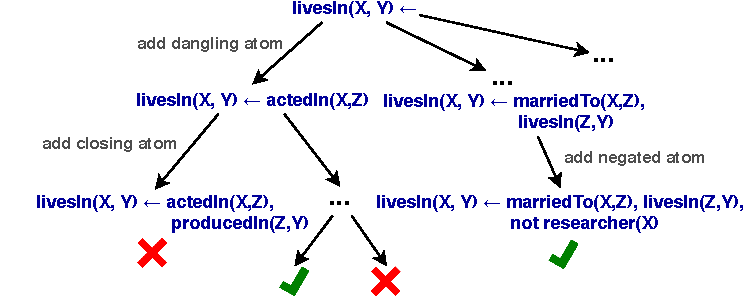
\includegraphics[width=.72\textwidth,height=16.5cm]{refinement_operators-crop}}
% 				\end{picture}
% 				\begin{columns}[t]
% 					\begin{column}{1.1\textwidth}
% 						% \small
%                                                 % Extend AMIE as follows:
% 						% \begin{itemize}
% 						% 	\item \textbf{\bl{Additional refinement operators}} plus:					
% 						% 	      \begin{itemize}
% Extensions compared to AMIE:

%                                 \begin{itemize}
%                                 \item Support for negated atoms
% 				\item Additional filtering criteria:
% 						\begin{itemize}
% 						      	      \item embedding-based measure ($\mu$)
% 						      	      \item exception confidence\\
% 						      	      \bl{\[e\textit{-}conf(r,\cG) = conf(r',\cG)\]}
% 							      	      where \gr{$r':body^-(r)\leftarrow body^+(r), not\;head(r)$} $\Rightarrow$ ensure the \bl{\textbf{quality of exceptions}}
% 							      \end{itemize}
% 							      \bigskip
% 				\end{itemize}
% 					\end{column}
% 					\begin{column}{0\textwidth}
% 					\end{column}					
% 				\end{columns}
						\begin{picture}(1.99,1.99)
					\put(325,-470){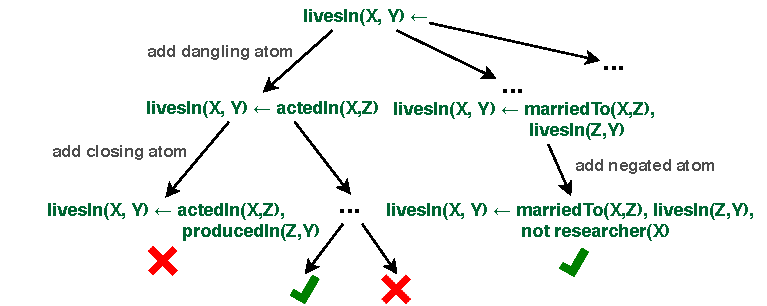
\includegraphics[width=.72\textwidth,height=16.5cm]{refinement_operators}}
				\end{picture}
				\begin{columns}[t]
					\begin{column}{1.1\textwidth}
						\small
						\vspace{-2.5em}
						\begin{itemize}
							\item \textbf{Refinement operators}: add					
							      \begin{itemize}
							      	\item  dangling atom
							      	      \medskip\item instantiated atom
							      	      \medskip\item closing atom
							      	      \medskip\item \textbf{\bl{negated instantiated atom}}
							      	      \medskip\item \textbf{\bl{negated closing atom}}
							      \end{itemize}
							      \bigskip\bigskip\bigskip
							\item \textbf{Rule filtering}:
							      \begin{itemize}
							      	\item language bias %rule form
							      	      \medskip\item support  
							      	      \medskip\item head coverage  
							      	      \medskip\item confidence  
							      	      \medskip\item \bl{\textbf{embedding-based measure ($\mu$)}} 
							      	      \medskip\item \textbf{\bl{exception confidence}}:
\vspace{-1cm}
\begin{center}
							      	      \bl{\[e\textit{-}conf(r,\cG) = conf(r',\cG)\]}
							      	      where \bl{$r':body^-(r)\leftarrow body^+(r), not\;head(r)$}\end{center}
							      \end{itemize}
							      \bigskip
						\end{itemize}
					\end{column}
					\begin{column}{0\textwidth}
					\end{column}					
				\end{columns}
	

			\end{block}
						
		\end{column}

		\begin{column}{0.5\textwidth}
\vspace{-.51cm}				
			\begin{block}{5. Experiments}
				\begin{picture}(1.99,1.99)
					\put(890,-200){
\includegraphics[width=.2\textwidth]{wikidata}}
				\end{picture}
				\begin{picture}(1.99,1.99)
					\put(500,-200){
\includegraphics[width=.23\textwidth]{freebase}}
				\end{picture}
				
				\begin{columns}
					\begin{column}{1.02\textwidth}
						\vspace{-1.7cm}
						\small{\begin{itemize}
							\item \bl{\textbf{Approximation of complete KG}}: original																		
							\item \bl{\textbf{Available KG}}: random 80\% of \\ original KG, preserving the distribution of facts over predicates.											\item \bl{\textbf{Embedding models}}: 
							\begin{itemize}
								\medskip
								\item TransE, HolE, SSP (with text)
							\end{itemize}
							\bigskip						
							%\item \bl{\textbf{Evaluation settings}}: \textit{closed world} setting (CW) and \textit{open world} setting (OW)							 
							\end{itemize}}
											
					
						\captionsetup[subfigure]{textfont=scriptsize}
						\begin{figure}[t]
							\centering
							%Gad: to unify legend and save space
							\subfloat{{
\includegraphics[width=0.5\textwidth]{figures/new_exp1/legend-crop.pdf} }}\\
							\setcounter{subfigure}{0}
							%     \subfloat[Conf-HolE on FB15K]{{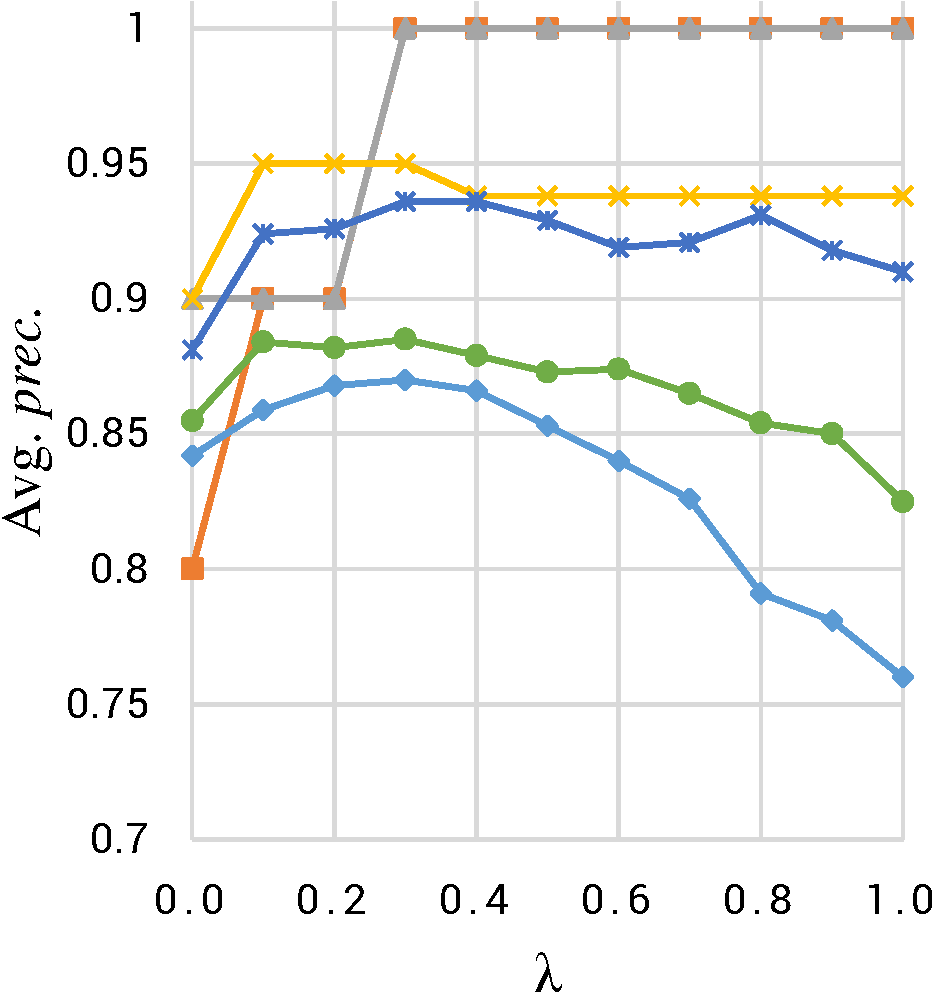
\includegraphics[width=0.3\textwidth]{figures/new_exp1/fb15k_hole_conf-crop.pdf} }\label{fig:fb-HoLE-Conf}}
							\subfloat[Conf-SSP on FB15K]{{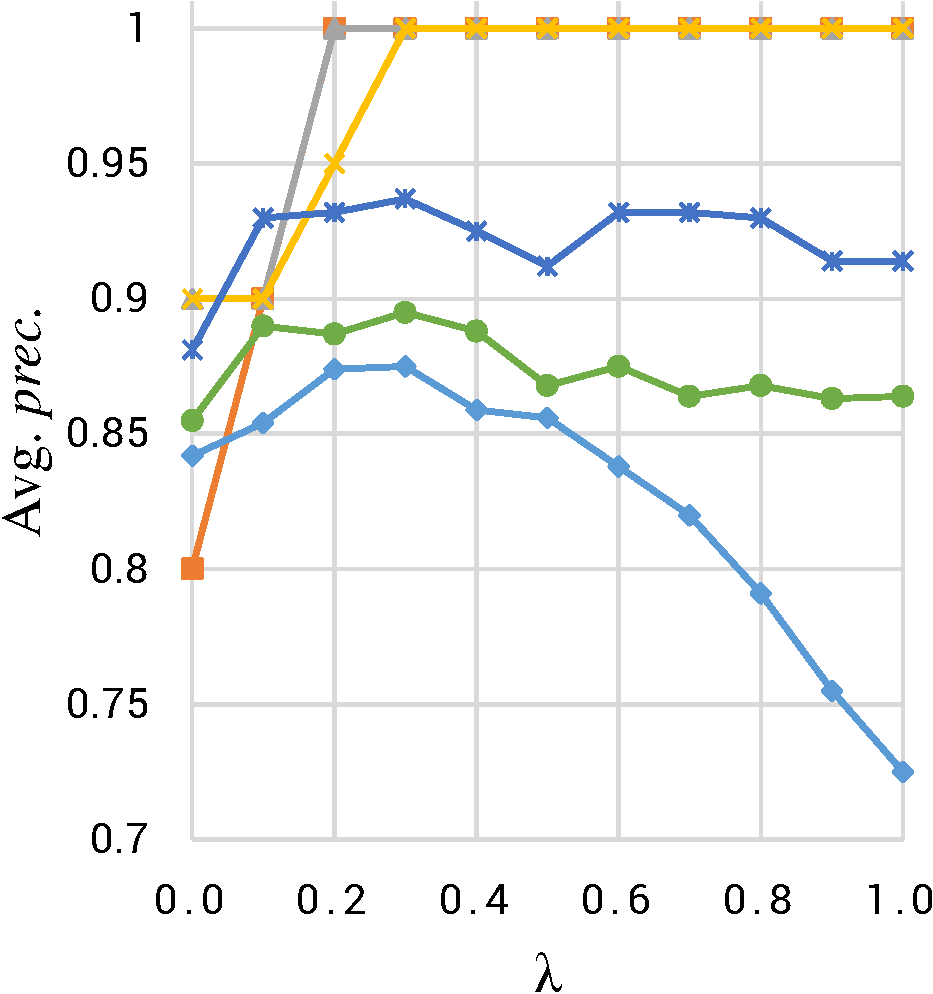
\includegraphics[width=0.24\textwidth]{figures/new_exp1/fb15k_ssp_conf-crop.pdf} \label{fig:fb-SSP-Conf}}}
							%\subfloat[RulES-H-PCA on FB15K]{{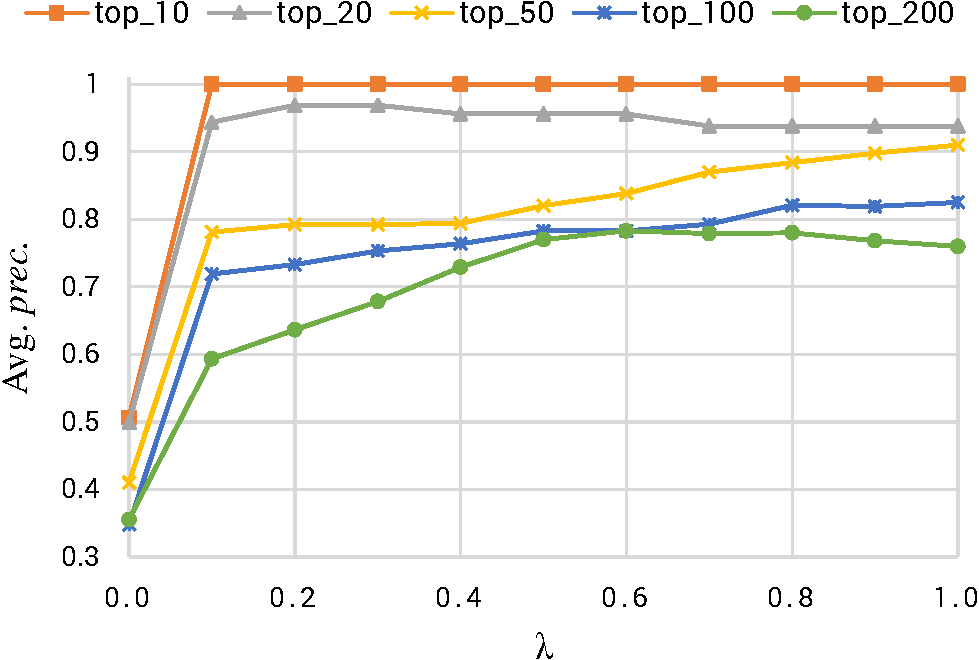
\includegraphics[width=0.3\textwidth]{figures/fb15k_hole_pca-crop.pdf} }}
							\subfloat[PCA-SSP on FB15K]{{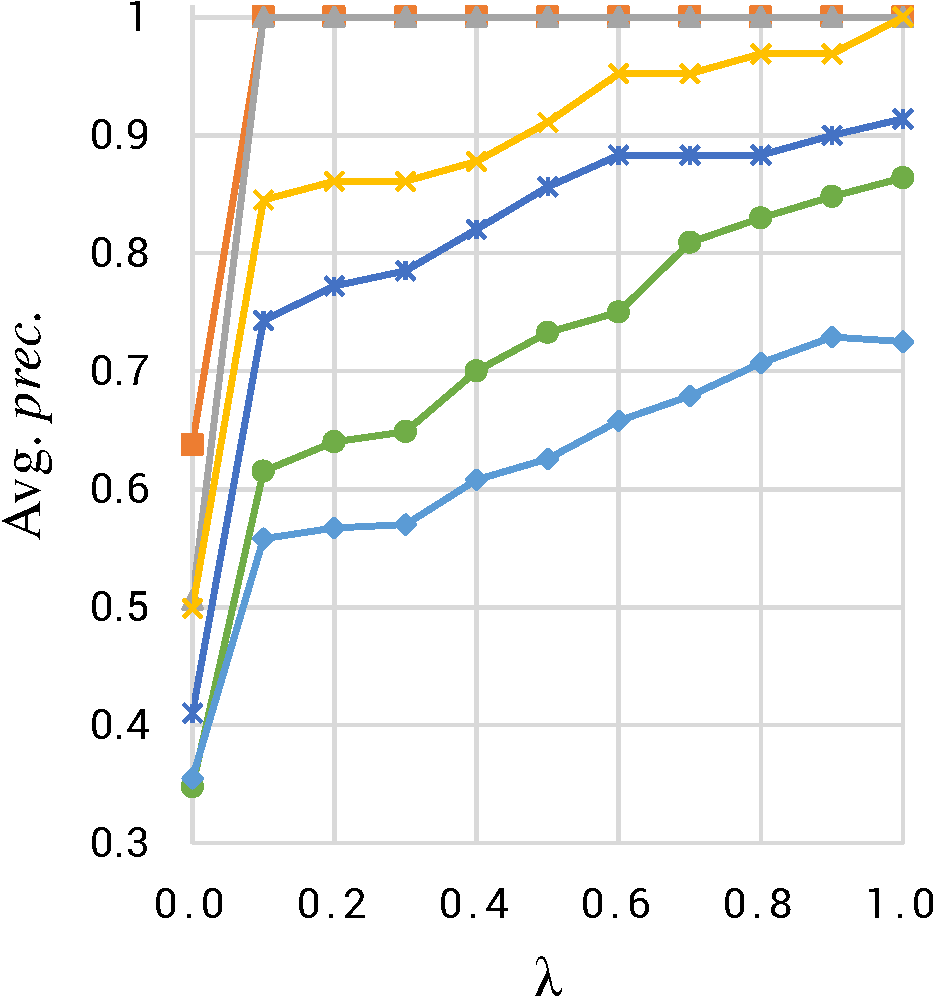
\includegraphics[width=0.24\textwidth]{figures/new_exp1/fb15k_ssp_pca-crop.pdf} }\label{fig:fb-SSP-PCA}}    
							%    \subfloat[Conf-TransE on Wiki44K]{{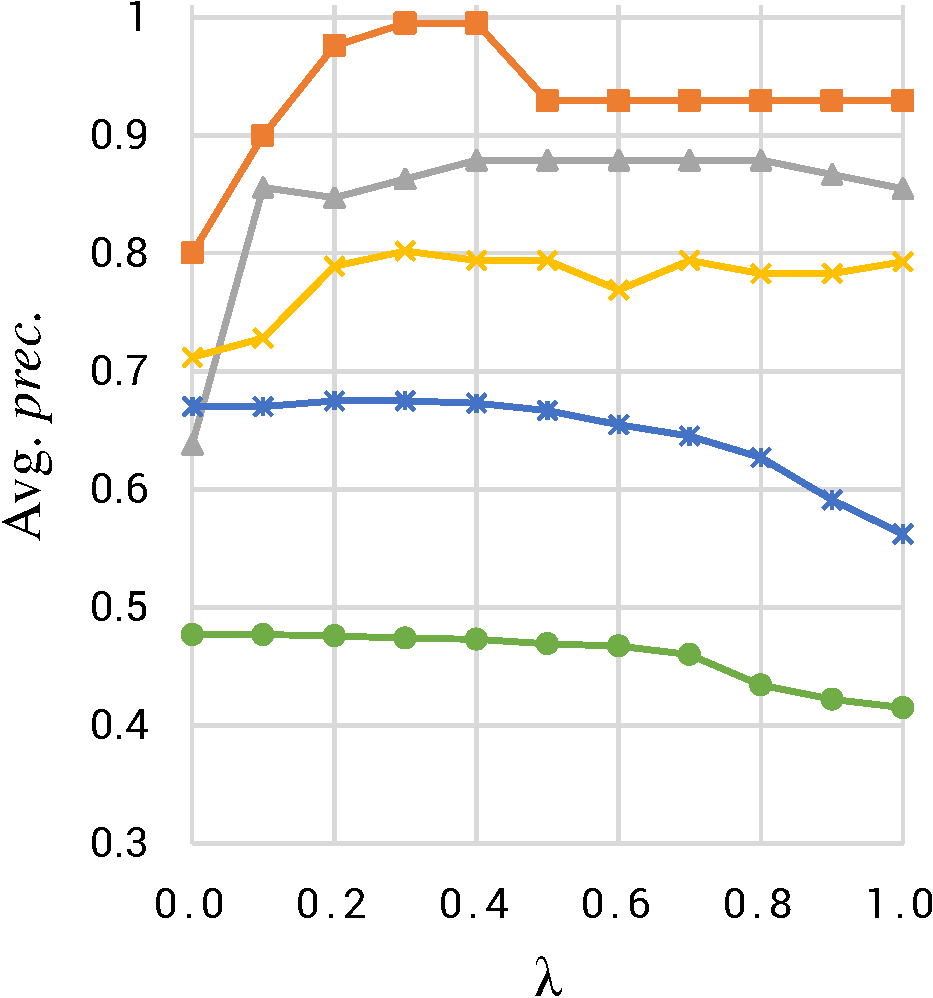
\includegraphics[width=0.3\textwidth]{figures/new_exp1/wiki44k_transe_conf-crop.pdf} }\label{fig:wi-TransE-Conf}}
							\subfloat[Conf-SSP on Wiki44K]{{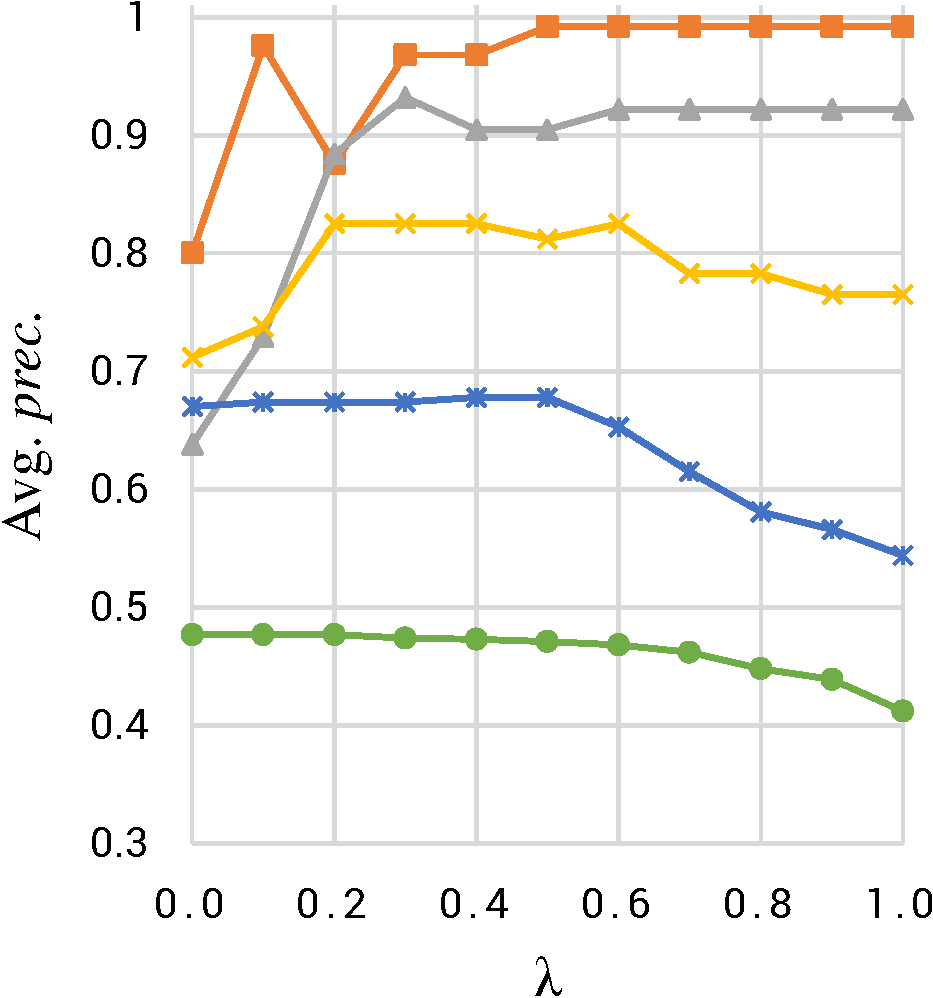
\includegraphics[width=0.24\textwidth]{figures/new_exp1/wiki44k_ssp_conf-crop.pdf} }\label{fig:wi-SSP-Conf}}
							%\subfloat[RulES-H-PCA on Wiki44K]{{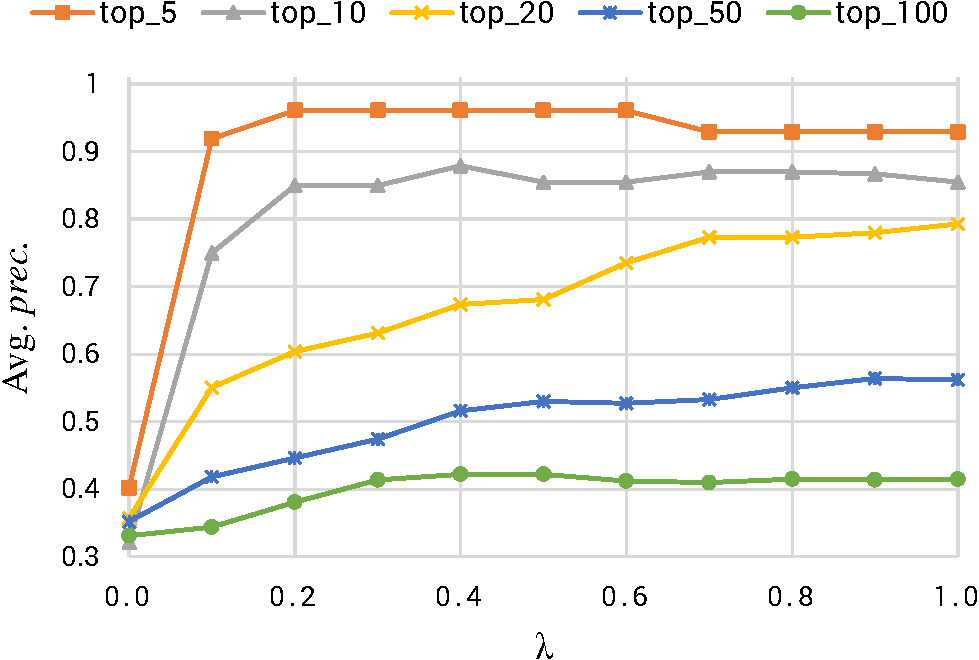
\includegraphics[width=0.3\textwidth]{figures/wiki44k_transe_pca-crop.pdf} }}
							\subfloat[PCA-SSP on Wiki44K]{{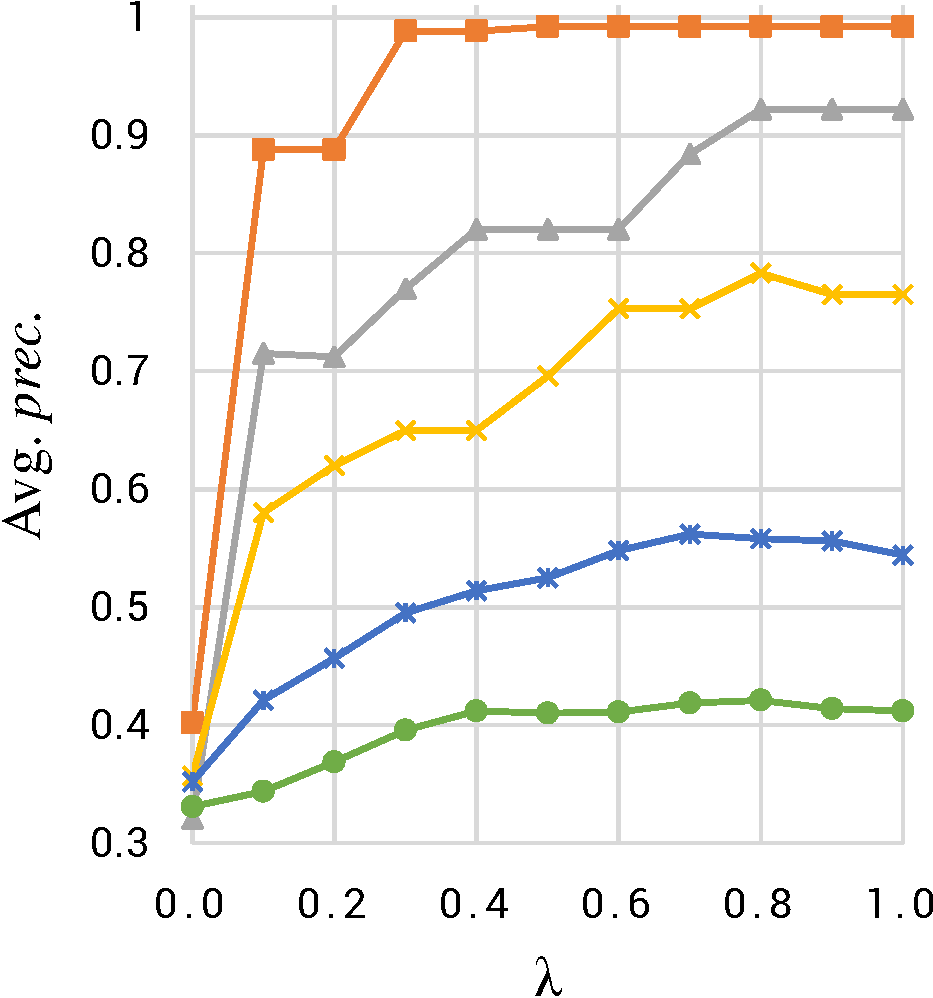
\includegraphics[width=0.24\textwidth]{figures/new_exp1/wiki44k_ssp_pca-crop.pdf} }\label{fig:wi-SSP-PCA}}
							    
							\caption{Evaluation result on \textit{closed world} setting (CW)}
							\label{fig:diff_lambda}
						\end{figure}
						\small
						\vspace{-0.8em}
						\begin{itemize}
							\item \textbf{\bl{Examples of mined rules:}}
							      
							      
							      				
							      \bigskip
							      				
							      \begin{tabular}{l}
							      	\small                                                                                                                              
							      	\gr{$r_1{:}$  $\mi{nationality(X{,}\, Y)}\, {\leftarrow}\, \mi{graduated\_from(X{,}\, Z)}{,}\, \mi{in\_country(Z{,}\, Y)},$}        
							      	\red{$not\ \mi{research\_uni(Z)}$}                                                                                                  \\
							      	\small                                                                                                                              
							      	\gr{$r_2{:}$  $\mi{scriptwriter\_of}(X{,}\, Y)\, {\leftarrow}\, \mi{preceded\_by(X{,}\, Z)}{,}\, \mi{scriptwriter\_of(Z{,}\, Y)},$} 
							      	\red{$not\ \mi{tv\_series(Z)}$}                                                                                                     
							      \end{tabular} 
						\end{itemize}

% \bl{\textbf{References}}
% 				\begin{thebibliography}{10}
% 					% \setlength{\itemsep}{0pt}
% 					\small{\footnotesize{	
%                                                 \bibitem[\protect\citeauthoryear{Galaraga \bgroup \em et al. \egroup
% 							}{2015}]{amie} L. Gal{\'{a}}rraga, C. Teflioudi, K. Hose, F. M. Suchanek.
% 						Fast Rule Mining in Ontol. KBs with AMIE+.{\em VLBD}, 2015.
%                                                   \bibitem[\protect\citeauthoryear{Wrobel}{1996}]{ilp}
% 						 D.~H.~Tran., D. Stepanova, M. Gad-Elrab, Francesca A. Lisi, G. Weikum. Towards Nonmonotonic Rule Learning from Knowledge Graphs. {\em Inductive Logic Programming}, 2016.				
% 						 \bibitem[\protect\citeauthoryear{V. T. Ho \bgroup \em et al. \egroup}{2018}]{ours}
% 						 V. T. Ho, D. Stepanova, M. Gad-Elrab, E. Kharlamov, G. Weikum. Rule Learning from Knowledge Graphs Guided by Embedding Models.
% 						 In proc. {\em International Semantic Web Conference}, 2018.
						
																		
						
					
% 					}}
										
										
										
										
% 				\end{thebibliography}
					\end{column}
					\begin{column}{.5\textwidth}
					\end{column}
				\end{columns}
			\end{block} 

						
		\end{column}
	\end{columns}
	\begin{columns}[t]
		\begin{column}{.5\textwidth}
			\vspace{-5cm}
			%\begin{block}{References}
								
			%\end{block}
						
		\end{column}
				
		\begin{column}{0.5\textwidth}
			%			\vspace{-6.7cm}
			%			\begin{block}{7. Further Work}
			%				\begin{itemize}
			%					\item \small{\textbf{\bl{Cardinality}} meta-data in \textbf{\bl{rule learning}}: \gr{John has \textbf{5} children, \textbf{3} people won award}}
			%				\end{itemize}
			%				\begin{columns}
			%					\begin{column}{.52\textwidth}
			%						\vspace{-.8cm}
			%						\begin{center}
			%							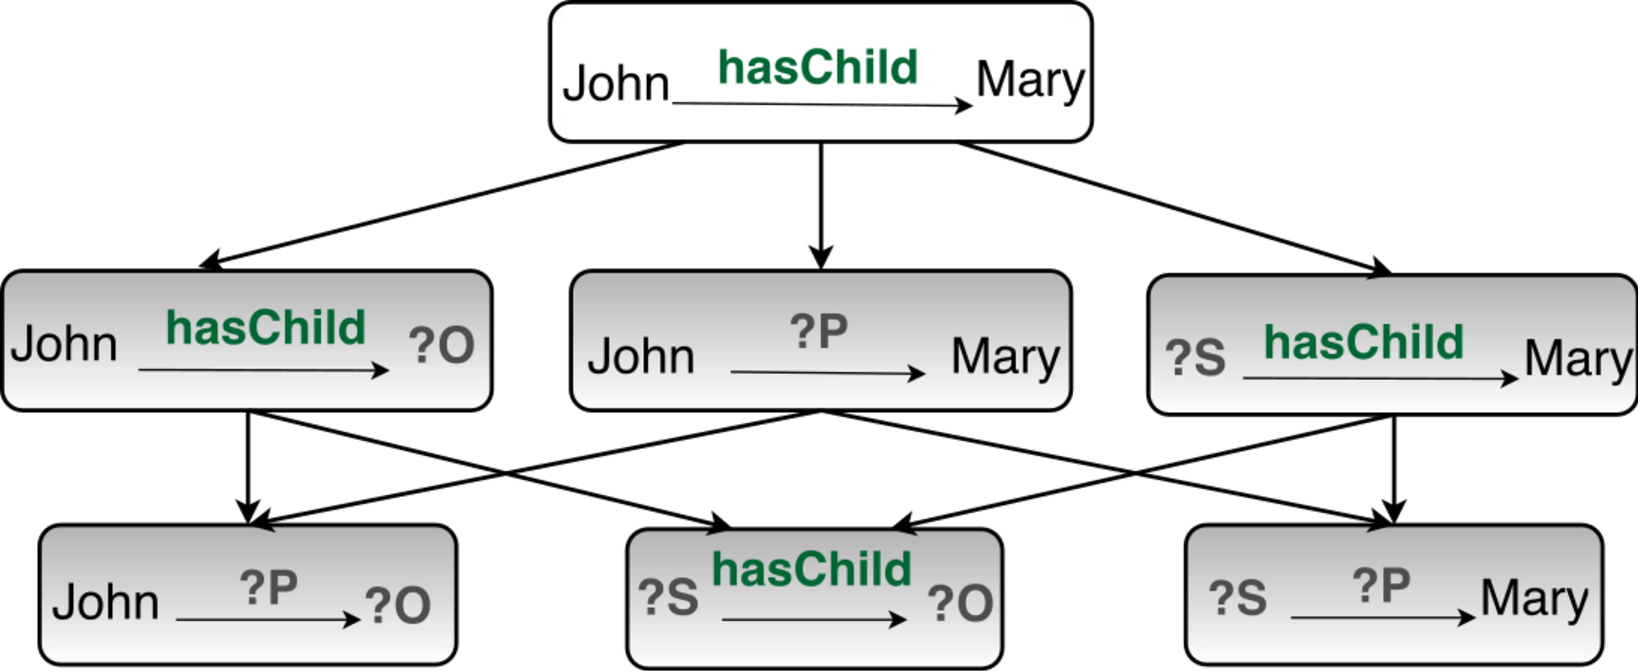
\includegraphics[width=.99\textwidth]{cs}
			%						\end{center}
			%					\end{column}
			%					\begin{column}{.48\textwidth}
			%						\vspace{-1.3cm}
			%						\begin{center}
			%							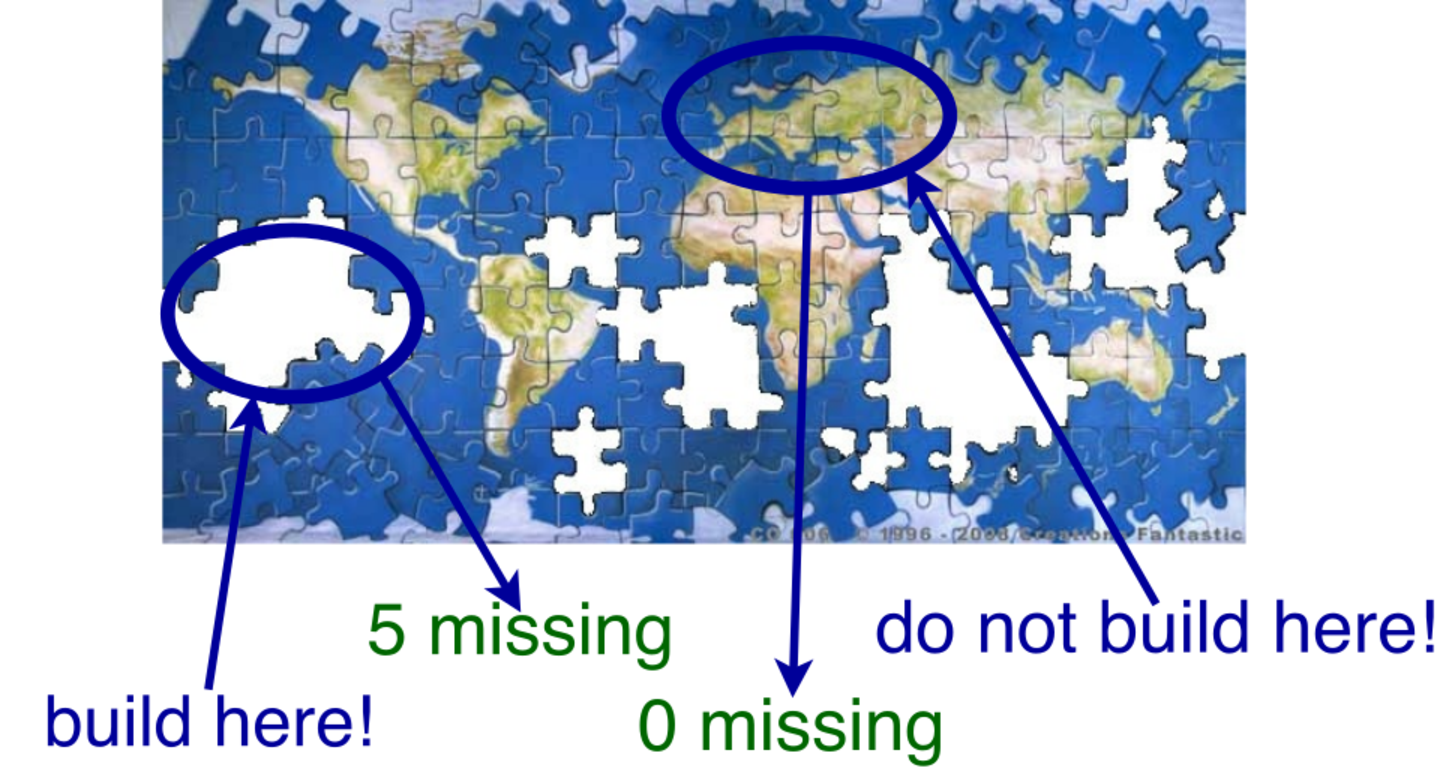
\includegraphics[width=.96\textwidth]{worldmap}
			%						\end{center}
			%					\end{column}
			%				\end{columns}
			%				\bigskip
			%				\bigskip
			%				
			%				\begin{itemize}
			%					\item \small{Learn \textbf{\bl{cardinality rules}}: \gr{``If X has $\leq$ 2 siblings, then his parents have $\leq$ 3 children''}}
			%				\end{itemize}
			%			\end{block}
		\end{column}
	\end{columns}
		
		 
		 
		
		
		
		
	\begin{tikzpicture}[remember picture,overlay]
		\node[] at (40.5,113.5) {%
			\begin{tabular}{c}
				\textbf{\huge{Learning Rules from Incomplete KGs}}                                                  \\
				\textbf{\huge{Using Embeddings \bigskip}}                                                                                     \\
				\bigskip \bigskip Vinh Thinh Ho$^1$, Daria Stepanova$^{1}$, Mohamed Gad-Elrab$^{1}$, Evgeny Kharlamov$^{2}$, Gerhard Weikum$^{1}$    \\
				\bigskip hvthinh@mpi-inf.mpg.de, dstepano@mpi-inf.mpg.de, gadelrab@mpi-inf.mpg.de, evgeny.kharlamov@cs.ox.ac.uk, weikum@mpi-inf.mpg.de \\
				$^1$Max Planck Institute for Informatics, Saarbr\"{u}cken, Germany                                                                     \\
				$^2$University of Oxford, Oxford, United Kingdom                                                                                       \\
				                                                                                                                                       
			\end{tabular}
		}; 
	\end{tikzpicture}
		
	\begin{tikzpicture}[remember picture,overlay]
		\node[] at (10.5,118) {%
			
\includegraphics[width=190mm]{mpi}%
		}; 
		% \node[] at (12,108) {%
		% 	
\includegraphics[width=70mm]{bosch}%
		% };
                
		\node[] at (75,118) {%
			
\includegraphics[height=42mm]{ox} 
		};
				
	\end{tikzpicture}
\end{frame}

\end{document}